% ============================================================
%  Network Security -- Module 7: Modern Block Ciphers and Modes of Operation
%  Lesson 13: IDEA
%  Lesson 14: Advanced Encryption Standard
%  Lesson 15: Modes of Operation
%  Beamer (Madrid theme). Compile with: pdflatex module7.tex (twice)
% ============================================================
\documentclass[aspectratio=169,11pt,xcolor={table}]{beamer}
\usetheme{Madrid}
\usefonttheme{professionalfonts}

\usepackage[T1]{fontenc}
\usepackage{lmodern}
\usepackage{booktabs}
\usepackage{array}
\usepackage{tikz}
\usetikzlibrary{arrows.meta,positioning,shapes.geometric,shapes.symbols,
  shapes.misc,shadows,calc,fit,backgrounds,mindmap,decorations.pathmorphing,decorations.pathreplacing}

% ------------------------------------------------------------
%  Colour palette
% ------------------------------------------------------------
\definecolor{navy}{RGB}{21,45,99}
\definecolor{ocean}{RGB}{28,97,158}
\definecolor{aqua}{RGB}{0,142,150}
\definecolor{brick}{RGB}{200,55,45}
\definecolor{amber}{RGB}{235,150,20}
\definecolor{leaf}{RGB}{40,160,90}
\definecolor{grape}{RGB}{125,70,165}
\definecolor{sky}{RGB}{235,243,252}
\definecolor{ink}{RGB}{40,40,50}

\setbeamercolor{palette primary}{bg=ocean,fg=white}
\setbeamercolor{palette secondary}{bg=navy!85,fg=white}
\setbeamercolor{palette tertiary}{bg=navy,fg=white}
\setbeamercolor{palette quaternary}{bg=navy,fg=white}
\setbeamercolor{structure}{fg=ocean}
\setbeamercolor{title}{bg=navy,fg=white}
\setbeamercolor{frametitle}{bg=navy,fg=white}
\setbeamercolor{block title}{bg=ocean,fg=white}
\setbeamercolor{block body}{bg=sky,fg=ink}
\setbeamercolor{block title alerted}{bg=brick,fg=white}
\setbeamercolor{block body alerted}{bg=brick!8,fg=ink}
\setbeamercolor{block title example}{bg=leaf,fg=white}
\setbeamercolor{block body example}{bg=leaf!8,fg=ink}
\setbeamercolor{normal text}{fg=ink}
\setbeamercolor{alerted text}{fg=brick}
\setbeamercolor{item projected}{bg=ocean,fg=white}
\setbeamertemplate{items}[circle]
\setbeamertemplate{blocks}[rounded][shadow=true]
\setbeamertemplate{navigation symbols}{}

% Section divider slide
\AtBeginSection[]{
  \begin{frame}[plain]
    \begin{tikzpicture}[remember picture,overlay]
      \fill[navy] (current page.south west) rectangle (current page.north east);
      \fill[ocean] (current page.south west) rectangle ([yshift=1.2cm]current page.south east);
      \fill[aqua] ([yshift=1.2cm]current page.south west) rectangle ([yshift=1.35cm]current page.south east);
      \foreach \i in {1,...,6}
        \draw[white,opacity=0.06,line width=14pt]
          ([xshift=\i*1.6cm]current page.north west) circle (\i*0.9cm);
      \node[white,font=\large,anchor=west] at ([xshift=1.2cm,yshift=0.9cm]current page.west)
        {Lesson \thesection};
      \node[white,font=\huge\bfseries,anchor=west,text width=12cm] at ([xshift=1.2cm,yshift=-0.1cm]current page.west)
        {\insertsectionhead};
      \node[white,opacity=0.8,anchor=east,font=\small] at ([xshift=-0.8cm,yshift=0.6cm]current page.south east)
        {Module 7 \,$\cdot$\, Modern Block Ciphers and Modes};
    \end{tikzpicture}
  \end{frame}
}

% ------------------------------------------------------------
%  TikZ styles and small pictograms
% ------------------------------------------------------------
\tikzset{
  >={Stealth[length=2.6mm]},
  box/.style={draw=#1!80!black,fill=#1!15,rounded corners=4pt,thick,
    minimum height=8mm,minimum width=22mm,align=center,font=\small,
    drop shadow={opacity=0.25}},
  box/.default=ocean,
  lay/.style={fill=#1,text=white,rounded corners=3pt,minimum width=38mm,minimum height=9mm,font=\scriptsize,align=center},
  solid box/.style={fill=#1,text=white,rounded corners=4pt,
    minimum height=8mm,minimum width=22mm,align=center,font=\small\bfseries,
    drop shadow={opacity=0.3}},
  solid box/.default=ocean,
  flow/.style={->,very thick,draw=#1},
  flow/.default=ink!70,
  station/.style={circle,draw=#1!80!black,fill=#1!20,very thick,minimum size=13mm,
    font=\small\bfseries,align=center},
  station/.default=ocean,
  tag/.style={font=\scriptsize,text=ink!80,align=center},
  layer/.style={draw=white,thick,fill=#1,text=white,minimum width=40mm,
    minimum height=6.5mm,font=\small\bfseries},
  % pictograms
  pics/pc/.style={code={
    \fill[#1!85!black,rounded corners=1.5pt] (-0.42,-0.05) rectangle (0.42,0.52);
    \fill[white!90!#1] (-0.36,0.01) rectangle (0.36,0.46);
    \fill[#1!85!black] (-0.06,-0.05) rectangle (0.06,-0.18);
    \fill[#1!85!black,rounded corners=1pt] (-0.24,-0.18) rectangle (0.24,-0.24);
  }},
  pics/pc/.default=ocean,
  pics/person/.style={code={
    \fill[#1] (0,0.46) circle (0.16);
    \fill[#1,rounded corners=5pt] (-0.27,-0.1) -- (-0.27,0.2) -- (0.27,0.2) -- (0.27,-0.1) -- cycle;
  }},
  pics/person/.default=ocean,
  pics/lock/.style={code={
    \draw[#1!80!black,line width=2.2pt] (-0.15,0.12) -- (-0.15,0.28) arc (180:0:0.15) -- (0.15,0.12);
    \fill[#1,rounded corners=2pt] (-0.26,-0.22) rectangle (0.26,0.14);
    \fill[white] (0,-0.02) circle (0.05);
    \fill[white] (-0.02,-0.02) rectangle (0.02,-0.13);
  }},
  pics/lock/.default=amber,
  pics/doc/.style={code={
    \fill[white,draw=#1,thick] (-0.25,-0.33) -- (-0.25,0.33) -- (0.12,0.33) -- (0.25,0.2) -- (0.25,-0.33) -- cycle;
    \draw[#1,thick] (0.12,0.33) -- (0.12,0.2) -- (0.25,0.2);
    \foreach \y in {0.12,0,-0.12,-0.24} \draw[#1!70,thick] (-0.16,\y) -- (0.16,\y);
  }},
  pics/doc/.default=ocean,
  pics/key/.style={code={
    \draw[#1,line width=2pt] (0,0) circle (0.12);
    \draw[#1,line width=2pt] (0.12,0) -- (0.5,0) (0.38,0) -- (0.38,-0.12) (0.47,0) -- (0.47,-0.1);
  }},
  pics/key/.default=amber,
}
\newcommand{\comma}{,}
\newcommand{\hl}[1]{\textcolor{ocean}{\textbf{#1}}}
\newcommand{\bad}[1]{\textcolor{brick}{\textbf{#1}}}
\newcommand{\good}[1]{\textcolor{leaf}{\textbf{#1}}}

\makeatletter
% University logo, small, top-right corner of every page
\AddToHook{shipout/foreground}{%
  \put(\strip@pt\paperwidth,0){%
    \makebox(0,0)[tr]{\raisebox{-0.8cm}{
\includegraphics[height=0.72cm]{au_logo.png}\hspace{0.15cm}}}}}
\makeatother

% ------------------------------------------------------------
\title[Module 7: Block Ciphers \& Modes]{Modern Block Ciphers and Modes of Operation}
\subtitle{Module 7 \,\textbar\, Lesson 13: IDEA \,\textbullet\, Lesson 14: AES \,\textbullet\, Lesson 15: Modes of Operation}
\author[Network Security]{Network Security}
\institute[SLM]{Self-Learning Material \,--\, Lessons 13, 14 \& 15}
\date{}

% 4x4 byte state grid: \stategrid{x}{y}{colour}{16 comma-separated entries, row by row}
\newcommand{\stategrid}[4]{%
  \foreach \v [count=\k from 0] in {#4}{
    \pgfmathtruncatemacro{\r}{\k/4}\pgfmathtruncatemacro{\c}{mod(\k,4)}
    \node[draw=#3,fill=#3!12,minimum size=6.5mm,font=\scriptsize\ttfamily,inner sep=0pt] at (#1+\c*0.65,#2-\r*0.65) {\v};
  }}

% block-cipher box used in the modes diagrams
\tikzset{ek/.style={solid box=navy,minimum width=13mm,minimum height=8mm,font=\scriptsize\bfseries},
  xorn/.style={circle,draw=navy,thick,inner sep=0pt,minimum size=5mm,font=\small},
  op/.style={circle,draw=#1,fill=#1!15,thick,minimum size=5.5mm,inner sep=0pt,font=\scriptsize},
  blk/.style={draw=#1,fill=#1!15,minimum width=12mm,minimum height=6mm,font=\scriptsize},blk/.default=leaf}

\begin{document}

% ============================================================
\begin{frame}[plain]
  
\begin{tikzpicture}[remember picture,overlay]
    \shade[top color=navy,bottom color=ocean] (current page.south west) rectangle (current page.north east);
    \foreach \i/\o in {1/0.10,2/0.08,3/0.06,4/0.05,5/0.04}
      \draw[white,opacity=\o,line width=1.2pt] ([xshift=-2.5cm,yshift=-0.5cm]current page.north east) circle (\i*1.1cm);
    \fill[aqua] ([yshift=2.35cm]current page.south west) rectangle ([yshift=2.45cm]current page.south east);
    \begin{scope}[shift={([xshift=-3.6cm,yshift=1.3cm]current page.east)}]
      \foreach \r in {0,...,3} \foreach \c in {0,...,3}{
        \pgfmathsetmacro{\o}{0.35+0.15*mod(\r+\c,4)}
        \fill[white,opacity=\o,rounded corners=1.5pt] (\c*0.55,-\r*0.55) rectangle ++(0.48,0.48);
      }
      \fill[amber,rounded corners=1.5pt] (0.55,-0.55) rectangle ++(0.48,0.48);
      \fill[amber,rounded corners=1.5pt] (1.65,-1.65) rectangle ++(0.48,0.48);
      \node[white,font=\scriptsize\bfseries] at (1.07,-2.05) {AES state};
    \end{scope}
    \node[white,anchor=west,font=\normalsize] at ([xshift=1.1cm,yshift=2.4cm]current page.west)
      {NETWORK SECURITY \,\textbar\, MODULE 7};
    \node[white,anchor=west,font=\fontsize{24}{29}\selectfont\bfseries,text width=10.5cm] at ([xshift=1.1cm,yshift=1.0cm]current page.west)
      {Modern Block Ciphers\\[2pt] and Modes of Operation};
    \node[white,opacity=0.9,anchor=west,text width=9cm,font=\small] at ([xshift=1.1cm,yshift=-0.9cm]current page.west)
      {Lesson 13 \,--\, IDEA\\ Lesson 14 \,--\, Advanced Encryption Standard\\ Lesson 15 \,--\, Modes of Operation};
    \node[white,opacity=0.85,anchor=west,font=\footnotesize] at ([xshift=1.1cm,yshift=1.2cm]current page.south west)
      {Add* \,$\cdot$\, Multiply* \,$\cdot$\, 52 sub-keys \,$\cdot$\, SubBytes \,$\cdot$\, ShiftRows \,$\cdot$\, MixColumns \,$\cdot$\, ECB \,$\cdot$\, CBC \,$\cdot$\, CFB \,$\cdot$\, OFB};
  \end{tikzpicture}
\end{frame}

% ============================================================
\begin{frame}{Roadmap of This Module}
  \centering
  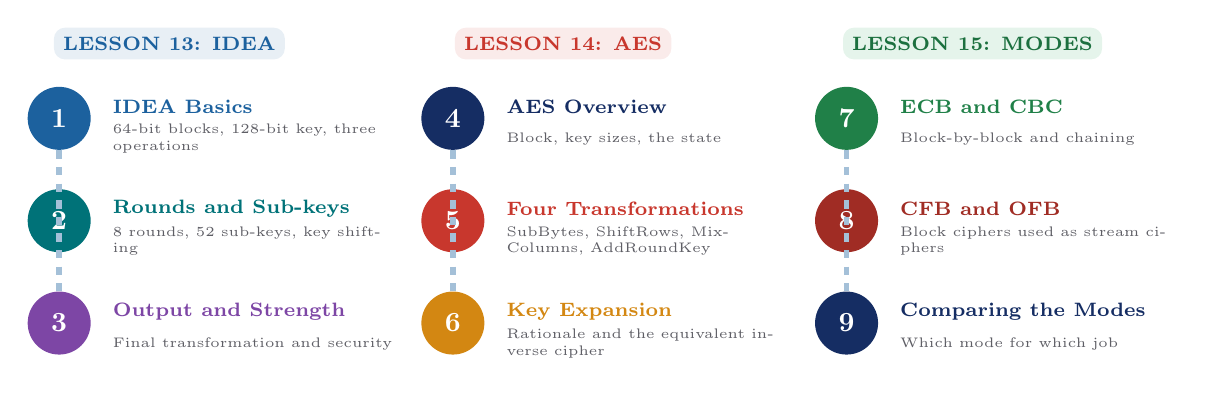
\begin{tikzpicture}
    \foreach \t/\c/\n/\x/\y [count=\i] in {
      IDEA Basics/ocean/64-bit blocks\comma{} 128-bit key\comma{} three operations/0/0,
      Rounds and Sub-keys/aqua!80!black/8 rounds\comma{} 52 sub-keys\comma{} key shifting/0/-1.3,
      Output and Strength/grape/Final transformation and security/0/-2.6,
      AES Overview/navy/Block\comma{} key sizes\comma{} the state/5.0/0,
      Four Transformations/brick/SubBytes\comma{} ShiftRows\comma{} MixColumns\comma{} AddRoundKey/5.0/-1.3,
      Key Expansion/amber!90!black/Rationale and the equivalent inverse cipher/5.0/-2.6,
      ECB and CBC/leaf!80!black/Block-by-block and chaining/10.0/0,
      CFB and OFB/brick!80!black/Block ciphers used as stream ciphers/10.0/-1.3,
      Comparing the Modes/navy/Which mode for which job/10.0/-2.6}
    {
      \node[circle,fill=\c,text=white,font=\bfseries,minimum size=8mm] (n\i) at (\x,\y) {\i};
      \node[anchor=west,font=\scriptsize\bfseries,text=\c] at ([xshift=1.5mm,yshift=1.5mm]n\i.east) {\t};
      \node[anchor=west,font=\tiny,text=ink!75,text width=36mm] at ([xshift=1.5mm,yshift=-2.6mm]n\i.east) {\n};
    }
    \draw[ocean!40,line width=2pt,dashed] (n1) -- (n3);
    \draw[ocean!40,line width=2pt,dashed] (n4) -- (n6);
    \draw[ocean!40,line width=2pt,dashed] (n7) -- (n9);
    \node[fill=ocean!10,rounded corners,font=\scriptsize\bfseries,text=ocean] at (1.4,0.95) {LESSON 13: IDEA};
    \node[fill=brick!10,rounded corners,font=\scriptsize\bfseries,text=brick] at (6.4,0.95) {LESSON 14: AES};
    \node[fill=leaf!12,rounded corners,font=\scriptsize\bfseries,text=leaf!70!black] at (11.6,0.95) {LESSON 15: MODES};
  \end{tikzpicture}
\end{frame}

% ============================================================
\setcounter{section}{12}
\section{IDEA}
% ============================================================

\begin{frame}{IDEA: International Data Encryption Algorithm}
  \begin{columns}[c]
    \begin{column}{0.5\textwidth}
      \centering
      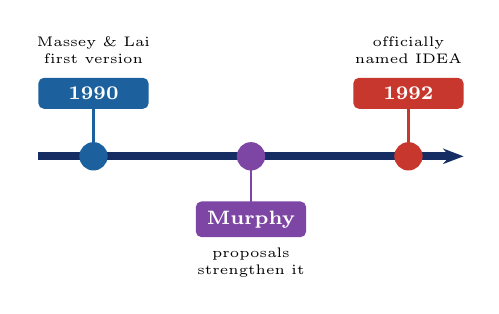
\begin{tikzpicture}
        \draw[navy,line width=3pt,->] (0,0) -- (5.4,0);
        \foreach \x/\c/\y/\t/\d in {0.7/ocean/1/1990/Massey \& Lai\\first version,2.7/grape/-1/Murphy/proposals\\strengthen it,4.7/brick/1/1992/officially\\named IDEA}{
          \fill[\c] (\x,0) circle (1.8mm); \draw[\c,thick] (\x,0) -- (\x,\y*0.6);
          \node[fill=\c,text=white,rounded corners=2pt,font=\scriptsize\bfseries,minimum width=14mm] at (\x,\y*0.8) {\t};
          \node[font=\tiny,align=center] at (\x,\y*1.35) {\d};
        }
      \end{tikzpicture}
    \end{column}
    \begin{column}{0.48\textwidth}
      \begin{itemize}\small\setlength{\itemsep}{3pt}
        \item Encrypts \textbf{64-bit} blocks using a \textbf{128-bit} key
        \item Based on three algebraic groups: \textbf{XOR}, \textbf{addition modulo $2^{16}$} and \textbf{multiplication modulo $2^{16}+1$}
        \item Unlike DES: \textbf{no permutations, no S-boxes}
        \item Used in the public-domain \textbf{Pretty Good Privacy (PGP)} e-mail system
      \end{itemize}
      \begin{exampleblock}{Why it was trusted}
        \small Secure against \textbf{differential cryptanalysis}, and its key is too long for exhaustive search.
      \end{exampleblock}
    \end{column}
  \end{columns}
\end{frame}

% ------------------------------------------------------------
\begin{frame}{Block Diagram of IDEA}
  \centering
  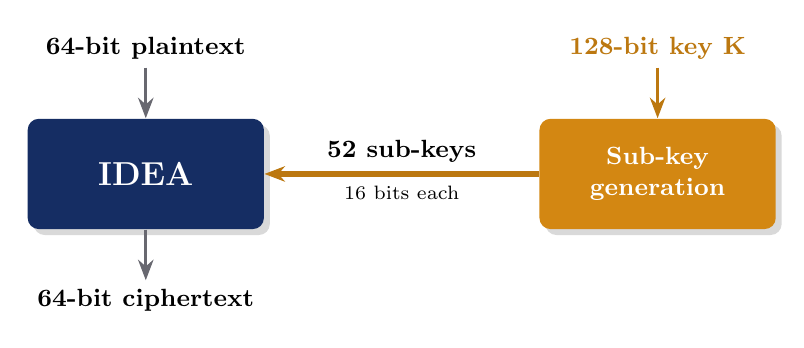
\begin{tikzpicture}
    \node[font=\small\bfseries] at (0,1.6) {64-bit plaintext};
    \node[solid box=navy,minimum width=30mm,minimum height=14mm,font=\large\bfseries] (idea) at (0,0) {IDEA};
    \node[font=\small\bfseries] at (0,-1.6) {64-bit ciphertext};
    \draw[flow] (0,1.35) -- (idea); \draw[flow] (idea) -- (0,-1.35);
    \node[font=\small\bfseries,text=amber!80!black] at (6.5,1.6) {128-bit key K};
    \node[solid box=amber!90!black,minimum width=30mm,minimum height=14mm,align=center] (sk) at (6.5,0) {Sub-key\\generation};
    \draw[flow=amber!80!black] (6.5,1.35) -- (sk);
    \draw[flow=amber!80!black,line width=2pt] (sk) -- node[above,font=\small\bfseries]{52 sub-keys} node[below,font=\scriptsize]{16 bits each} (idea);
  \end{tikzpicture}
  \vspace{4mm}
  \begin{block}{Basic principles}
    \small IDEA is a \textbf{symmetric block cipher}. Like DES it works on 64-bit blocks and is \textbf{reversible} (the same algorithm encrypts and decrypts), and uses both \textbf{diffusion and confusion}. But its round function and sub-key generation are very different from DES.
  \end{block}
\end{frame}

% ------------------------------------------------------------
\begin{frame}{The Three Operations of IDEA}
  \centering
  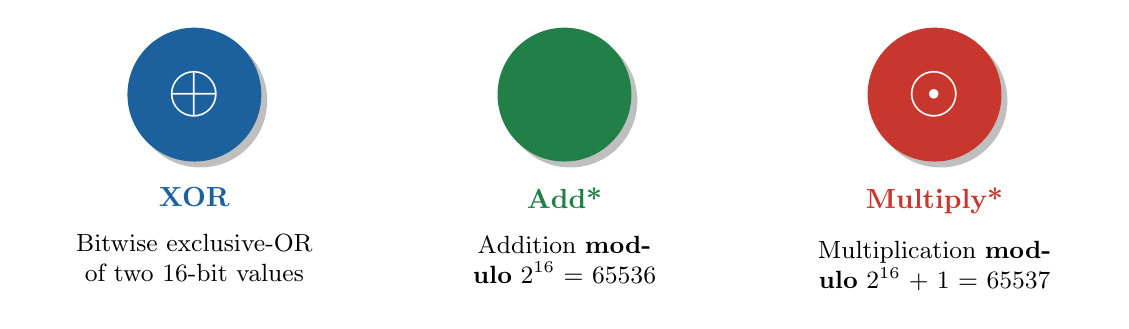
\begin{tikzpicture}
    \foreach \x/\c/\s/\t/\d in {
      0/ocean/$\oplus$/XOR/Bitwise exclusive-OR of two 16-bit values,
      4.7/leaf!80!black/$\boxplus$/Add*/Addition \textbf{modulo $2^{16}$} = 65536,
      9.4/brick/$\odot$/Multiply*/Multiplication \textbf{modulo $2^{16}+1$} = 65537}
    {
      \node[circle,fill=\c,text=white,font=\Huge,minimum size=17mm,drop shadow] (c) at (\x,0) {\s};
      \node[font=\bfseries,text=\c,below=2mm of c] (t) {\t};
      \node[font=\small,text width=40mm,align=center,below=1mm of t] {\d};
    }
  \end{tikzpicture}
  \vspace{4mm}
  \begin{alertblock}{Why the asterisk?}
    \small Add* and Multiply* are \textbf{not ordinary} addition and multiplication. Results are reduced with \textbf{mod} so they always fit in 16 bits. ($a \bmod b$ is the remainder of $a/b$: $5 \bmod 2 = 1$, $5 \bmod 3 = 2$.)
  \end{alertblock}
\end{frame}

% ------------------------------------------------------------
\begin{frame}{Why Modulo? A Worked Example (Fig.\ 13.4)}
  \begin{columns}[c]
    \begin{column}{0.54\textwidth}
      \centering
      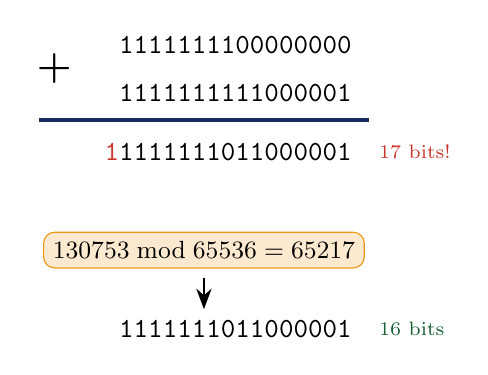
\begin{tikzpicture}
        \node[font=\ttfamily,anchor=east] at (3.6,1.2) {1111111100000000};
        \node[font=\ttfamily,anchor=east] at (3.6,0.6) {1111111111000001};
        \node[font=\Large\bfseries] at (-0.3,0.9) {+};
        \draw[navy,very thick] (-0.5,0.25) -- (3.7,0.25);
        \node[font=\ttfamily,anchor=east] at (3.6,-0.15) {\textcolor{brick}{\textbf{1}}1111111011000001};
        \node[font=\scriptsize,text=brick,anchor=west] at (3.7,-0.15) {17 bits!};
        \node[fill=amber!20,draw=amber,rounded corners,font=\small,align=center] at (1.6,-1.4) {$130753 \bmod 65536 = 65217$};
        \node[font=\ttfamily,anchor=east] at (3.6,-2.4) {1111111011000001};
        \node[font=\scriptsize,text=leaf!60!black,anchor=west] at (3.7,-2.4) {16 bits};
        \draw[->,thick] (1.6,-1.75) -- (1.6,-2.15);
      \end{tikzpicture}
    \end{column}
    \begin{column}{0.44\textwidth}
      \begin{itemize}\small\setlength{\itemsep}{4pt}
        \item In round 2, suppose $P_2$ = \texttt{1111111100000000} and $K_2$ = \texttt{1111111111000001}
        \item Ordinary addition gives a \textbf{17-bit} result (130753)
        \item Only \textbf{16 bit positions} are available
        \item Taking mod 65536 gives 65217, which fits in 16 bits
      \end{itemize}
      \begin{block}{So}
        \small Modulo arithmetic brings every result \textbf{back to 16 bits}.
      \end{block}
    \end{column}
  \end{columns}
\end{frame}

% ------------------------------------------------------------
\begin{frame}{Broad-Level Steps (Fig.\ 13.2)}
  \begin{columns}[c]
    \begin{column}{0.52\textwidth}
      \centering
      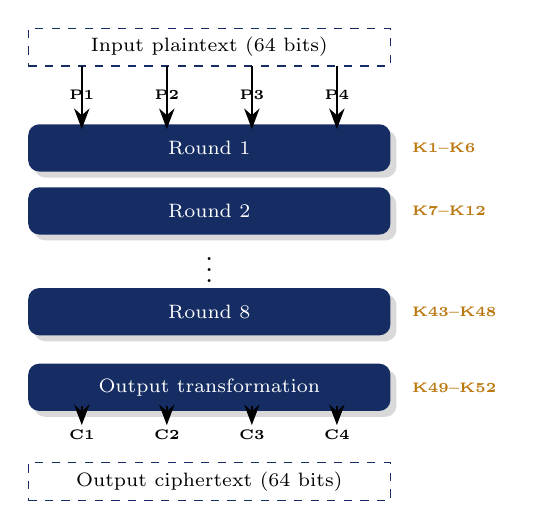
\begin{tikzpicture}[y=0.8cm]
        \node[draw=navy,dashed,minimum width=46mm,font=\scriptsize] (pt) at (0,0.6) {Input plaintext (64 bits)};
        \foreach \i in {1,...,4} \node[font=\tiny\bfseries] at (-2.7+\i*1.08,-0.15) {P\i};
        \foreach \t/\y/\k [count=\i] in {Round 1/-1/K1--K6,Round 2/-2/K7--K12,Round 8/-3.6/K43--K48,Output transformation/-4.8/K49--K52}{
          \node[solid box=navy,minimum width=46mm,minimum height=6mm,font=\scriptsize] (r\i) at (0,\y) {\t};
          \node[font=\tiny\bfseries,text=amber!80!black,anchor=west] at (2.45,\y) {\k};
        }
        \node at (0,-2.8) {$\vdots$};
        \foreach \i in {1,...,4} \node[font=\tiny\bfseries] at (-2.7+\i*1.08,-5.55) {C\i};
        \node[draw=navy,dashed,minimum width=46mm,font=\scriptsize] at (0,-6.3) {Output ciphertext (64 bits)};
        \foreach \i in {1,...,4}{ \draw[->,thick] (-2.7+\i*1.08,0.3) -- (-2.7+\i*1.08,-0.7); \draw[->,thick] (-2.7+\i*1.08,-5.1) -- (-2.7+\i*1.08,-5.4);}
      \end{tikzpicture}
    \end{column}
    \begin{column}{0.46\textwidth}
      \begin{enumerate}\small\setlength{\itemsep}{3pt}
        \item The 64-bit block is split into four \textbf{16-bit} parts, P1--P4
        \item There are \textbf{8 rounds}; each uses \textbf{6 sub-keys}
        \item Round 1 uses K1--K6, round 2 uses K7--K12, \dots, round 8 uses K43--K48
        \item A final \textbf{output transformation} uses 4 sub-keys, K49--K52
        \item Its output, C1--C4, forms the 64-bit ciphertext
      \end{enumerate}
      \begin{block}{Count}
        \small $8 \times 6 + 4 = $ \textbf{52 sub-keys}
      \end{block}
    \end{column}
  \end{columns}
\end{frame}

% ------------------------------------------------------------
\begin{frame}{The 14 Steps of One Round (Fig.\ 13.3)}
  \centering
  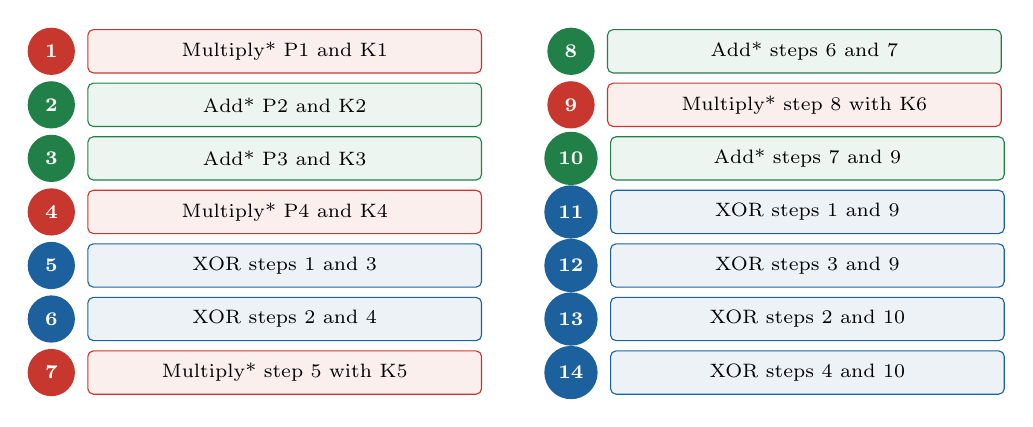
\begin{tikzpicture}
    \foreach \t/\c [count=\i] in {
      Multiply* P1 and K1/brick,Add* P2 and K2/leaf!80!black,Add* P3 and K3/leaf!80!black,Multiply* P4 and K4/brick,
      XOR steps 1 and 3/ocean,XOR steps 2 and 4/ocean,Multiply* step 5 with K5/brick,
      Add* steps 6 and 7/leaf!80!black,Multiply* step 8 with K6/brick,Add* steps 7 and 9/leaf!80!black,
      XOR steps 1 and 9/ocean,XOR steps 3 and 9/ocean,XOR steps 2 and 10/ocean,XOR steps 4 and 10/ocean}
    {
      \pgfmathsetmacro{\x}{ifthenelse(\i<8,0,6.6)}
      \pgfmathsetmacro{\y}{-mod(\i-1,7)*0.68}
      \node[circle,fill=\c,text=white,font=\scriptsize\bfseries,minimum size=6mm] (s\i) at (\x,\y) {\i};
      \node[draw=\c,fill=\c!8,rounded corners=2pt,anchor=west,minimum width=50mm,minimum height=5.5mm,font=\scriptsize] at ([xshift=1.5mm]s\i.east) {\t};
    }
  \end{tikzpicture}
  \vspace{2mm}

  {\small Steps 1--4 mix the four inputs with K1--K4; steps 5--10 form the ``MA'' structure with K5 and K6; steps 11--14 give R1--R4. \textcolor{brick}{\textbf{Multiply*}}, \textcolor{leaf!70!black}{\textbf{Add*}}, \textcolor{ocean}{\textbf{XOR}}.}
\end{frame}

% ------------------------------------------------------------
\begin{frame}{One Round of IDEA (Fig.\ 13.5)}
  \begin{columns}[c]
    \begin{column}{0.58\textwidth}
      \centering
      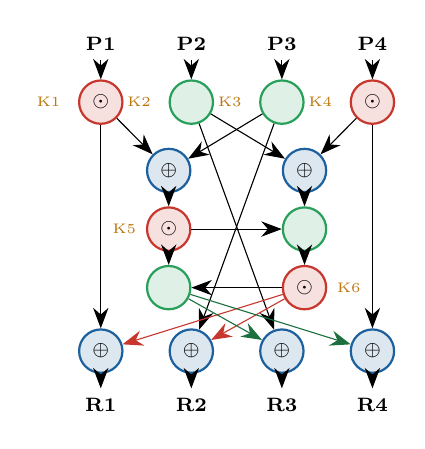
\begin{tikzpicture}[x=1.15cm,y=0.62cm]
        \foreach \i/\x in {1/0,2/1,3/2,4/3} \node[font=\scriptsize\bfseries] (P\i) at (\x,0.6) {P\i};
        \node[op=brick] (m1) at (0,-0.6) {$\odot$}; \node[op=leaf] (a2) at (1,-0.6) {$\boxplus$};
        \node[op=leaf] (a3) at (2,-0.6) {$\boxplus$}; \node[op=brick] (m4) at (3,-0.6) {$\odot$};
        \foreach \k/\n in {1/m1,2/a2,3/a3,4/m4} \node[font=\tiny,text=amber!80!black,anchor=east] at ([xshift=-1mm]\n.west) {K\k};
        \foreach \i/\n in {1/m1,2/a2,3/a3,4/m4} \draw[->] (P\i) -- (\n);
        \node[op=ocean] (x5) at (0.75,-2) {$\oplus$}; \node[op=ocean] (x6) at (2.25,-2) {$\oplus$};
        \draw[->] (m1) -- (x5); \draw[->] (a3) -- (x5); \draw[->] (a2) -- (x6); \draw[->] (m4) -- (x6);
        \node[op=brick] (m7) at (0.75,-3.2) {$\odot$}; \node[font=\tiny,text=amber!80!black,anchor=east] at (m7.west) {K5};
        \node[op=leaf] (a8) at (2.25,-3.2) {$\boxplus$};
        \node[op=brick] (m9) at (2.25,-4.4) {$\odot$}; \node[font=\tiny,text=amber!80!black,anchor=west] at (m9.east) {K6};
        \node[op=leaf] (a10) at (0.75,-4.4) {$\boxplus$};
        \draw[->] (x5) -- (m7); \draw[->] (x6) -- (a8); \draw[->] (m7) -- (a8); \draw[->] (a8) -- (m9); \draw[->] (m9) -- (a10); \draw[->] (m7) -- (a10);
        \foreach \i/\x in {1/0,2/1,3/2,4/3} \node[op=ocean] (o\i) at (\x,-5.7) {$\oplus$};
        \draw[->] (m1) -- (o1); \draw[->] (a3) -- (o2); \draw[->] (a2) -- (o3); \draw[->] (m4) -- (o4);
        \draw[->,brick] (m9) -- (o1); \draw[->,brick] (m9) -- (o2); \draw[->,leaf!70!black] (a10) -- (o3); \draw[->,leaf!70!black] (a10) -- (o4);
        \foreach \i/\x in {1/0,2/1,3/2,4/3} {\node[font=\scriptsize\bfseries] (R\i) at (\x,-6.8) {R\i}; \draw[->] (o\i) -- (R\i);}
      \end{tikzpicture}
    \end{column}
    \begin{column}{0.4\textwidth}
      \begin{itemize}\small\setlength{\itemsep}{3pt}
        \item Same steps as before, drawn \textbf{symbolically}
        \item Inputs P1--P4, sub-keys K1--K6, outputs \textbf{R1--R4}
        \item R1--R4 are \textbf{not} the final ciphertext: they feed the next round, or the output transformation
        \item Note R2 and R3 are \textbf{swapped} in the middle blocks
      \end{itemize}
      \begin{block}{Legend}
        \small $\odot$ Multiply* \quad $\boxplus$ Add* \quad $\oplus$ XOR
      \end{block}
    \end{column}
  \end{columns}
\end{frame}

% ------------------------------------------------------------
\begin{frame}{Sub-Key Generation: Rounds 1 and 2}
  \centering
  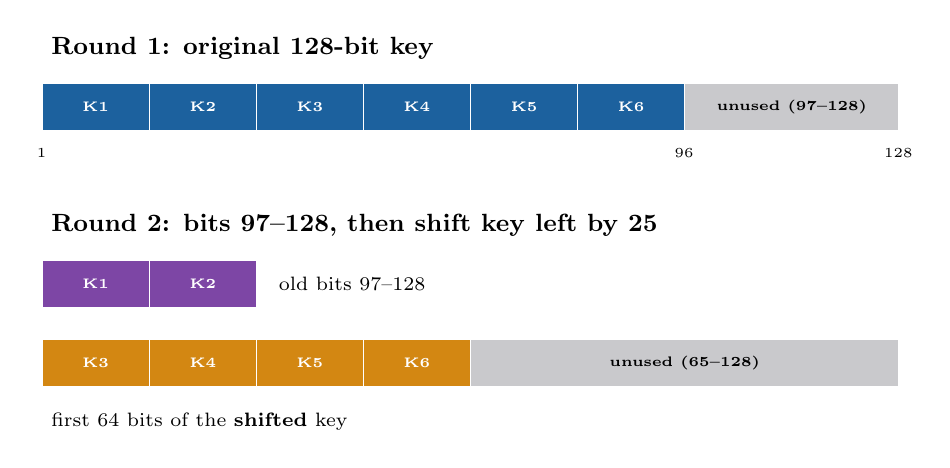
\begin{tikzpicture}[x=0.85mm]
    \node[font=\small\bfseries,anchor=west] at (0,0.75) {Round 1: original 128-bit key};
    \foreach \i [count=\k from 0] in {1,...,6} \node[draw=white,fill=ocean,text=white,font=\tiny\bfseries,minimum width=13.6mm,minimum height=6mm,anchor=west] at (\k*16,0) {K\i};
    \node[draw=white,fill=ink!25,font=\tiny\bfseries,minimum width=27.2mm,minimum height=6mm,anchor=west] at (96,0) {unused (97--128)};
    \foreach \b/\x in {1/0,96/96,128/128} \node[font=\tiny,anchor=north] at (\x,-0.4) {\b};
    \node[font=\small\bfseries,anchor=west] at (0,-1.5) {Round 2: bits 97--128, then shift key \textbf{left by 25}};
    \node[draw=white,fill=grape,text=white,font=\tiny\bfseries,minimum width=13.6mm,minimum height=6mm,anchor=west] at (0,-2.25) {K1};
    \node[draw=white,fill=grape,text=white,font=\tiny\bfseries,minimum width=13.6mm,minimum height=6mm,anchor=west] at (16,-2.25) {K2};
    \node[font=\scriptsize,anchor=west] at (34,-2.25) {old bits 97--128};
    \foreach \i [count=\k from 0] in {3,...,6} \node[draw=white,fill=amber!90!black,text=white,font=\tiny\bfseries,minimum width=13.6mm,minimum height=6mm,anchor=west] at (\k*16,-3.25) {K\i};
    \node[draw=white,fill=ink!25,font=\tiny\bfseries,minimum width=54.4mm,minimum height=6mm,anchor=west] at (64,-3.25) {unused (65--128)};
    \node[font=\scriptsize,anchor=west] at (0,-4.0) {first 64 bits of the \textbf{shifted} key};
  \end{tikzpicture}
  \vspace{2mm}
  \begin{itemize}\small
    \item Round 1 uses bits \textbf{1--96} (6 sub-keys $\times$ 16 bits); bits 97--128 are left over
    \item Round 2 needs 96 bits: 32 left over + 64 more. The key is \textbf{circular-left shifted by 25 bits}: bit 26 becomes bit 1, bit 25 becomes bit 128
  \end{itemize}
\end{frame}

% ------------------------------------------------------------
\begin{frame}{Sub-Key Generation for All Rounds (Table 13.2)}
  \centering
  \renewcommand{\arraystretch}{1.3}
  \small
  \begin{tabular}{c >{\raggedright\arraybackslash}p{4.2cm} >{\raggedright\arraybackslash}p{4.2cm} c}
    \toprule
    \rowcolor{navy}\textcolor{white}{\textbf{Round}} & \textcolor{white}{\textbf{Sub-keys from current key}} & \textcolor{white}{\textbf{Then}} & \textcolor{white}{\textbf{Left over}}\\
    \midrule
    1, 5 & Bits 1--96 $\rightarrow$ K1--K6 & --- & 97--128\\
    2, 6 & Bits 97--128 $\rightarrow$ K1, K2 & Shift 25; bits 1--64 $\rightarrow$ K3--K6 & 65--128\\
    3, 7 & Bits 65--128 $\rightarrow$ K1--K4 & Shift 25; bits 1--32 $\rightarrow$ K5, K6 & 33--128\\
    4, 8 & Bits 33--128 $\rightarrow$ K1--K6 & Shift 25 & none\\
    Output & Bits 1--64 $\rightarrow$ K1--K4 & --- & ---\\
    \bottomrule
  \end{tabular}
  \vspace{4mm}

  
\begin{tikzpicture}
    \node[fill=sky,rounded corners,text width=12cm,align=center,font=\small,inner sep=6pt]
      {Every round takes \textbf{96 bits} this way. The pattern repeats every 4 rounds, and at the end of round 8 \textbf{no bits are unused}.};
  \end{tikzpicture}
\end{frame}

% ------------------------------------------------------------
\begin{frame}{Output Transformation (Figs.\ 13.8 and 13.9)}
  \begin{columns}[c]
    \begin{column}{0.5\textwidth}
      \centering
      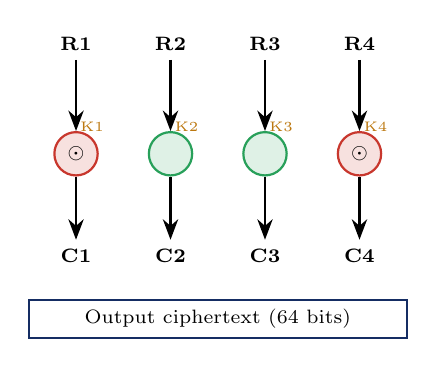
\begin{tikzpicture}[x=1.2cm]
        \foreach \i/\x in {1/0,2/1,3/2,4/3} \node[font=\scriptsize\bfseries] (R\i) at (\x,1.4) {R\i};
        \node[op=brick] (a) at (0,0) {$\odot$}; \node[op=leaf] (b) at (1,0) {$\boxplus$};
        \node[op=leaf] (c) at (2,0) {$\boxplus$}; \node[op=brick] (d) at (3,0) {$\odot$};
        \foreach \k/\n in {1/a,2/b,3/c,4/d} \node[font=\tiny,text=amber!80!black,anchor=south] at ([yshift=-0.5mm]\n.north east) {K\k};
        \foreach \i/\n in {1/a,2/b,3/c,4/d} \draw[->,thick] (R\i) -- (\n);
        \foreach \i/\n/\x in {1/a/0,2/b/1,3/c/2,4/d/3} {\node[font=\scriptsize\bfseries] (C\i) at (\x,-1.3) {C\i}; \draw[->,thick] (\n) -- (C\i);}
        \node[draw=navy,thick,minimum width=48mm,font=\scriptsize] at (1.5,-2.1) {Output ciphertext (64 bits)};
      \end{tikzpicture}
    \end{column}
    \begin{column}{0.48\textwidth}
      \begin{itemize}\small\setlength{\itemsep}{3pt}
        \item A \textbf{one-time} operation after round 8
        \item Input: round 8's output, R1--R4 (four 16-bit blocks)
        \item Uses \textbf{4 sub-keys}, not 6
      \end{itemize}
      \begin{block}{Four steps}
        \small 1.~Multiply* R1 and K1 \\ 2.~Add* R2 and K2 \\ 3.~Add* R3 and K3 \\ 4.~Multiply* R4 and K4
      \end{block}
      {\small Its sub-keys: after round 8 the key is shifted by 25 again, and the \textbf{first 64 bits} become K1--K4.}
    \end{column}
  \end{columns}
\end{frame}

% ------------------------------------------------------------
\begin{frame}{IDEA Decryption and Strength}
  \begin{columns}[T]
    \begin{column}{0.48\textwidth}
      \begin{block}{Decryption}
        \small Exactly the \textbf{same process} as encryption, with changes in the generation and pattern of sub-keys: the decryption sub-keys are the \textbf{inverses} of the encryption sub-keys.
      \end{block}
      \centering
      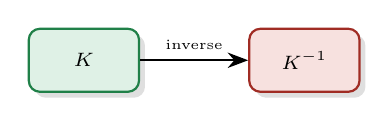
\begin{tikzpicture}
        \node[box=leaf,minimum width=14mm,font=\scriptsize] (k) at (0,0) {$K$};
        \node[box=brick,minimum width=14mm,font=\scriptsize] (ki) at (2.8,0) {$K^{-1}$};
        \draw[->,thick] (k) -- node[above,font=\tiny]{inverse} (ki);
      \end{tikzpicture}
    \end{column}
    \begin{column}{0.5\textwidth}
      \begin{alertblock}{Strength}
        \small A \textbf{128-bit} key, double the size of DES. Brute force needs $2^{128} \approx 10^{38}$ operations.
      \end{alertblock}
      \centering
      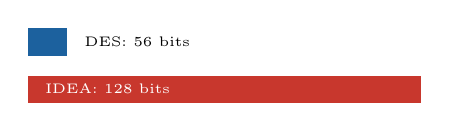
\begin{tikzpicture}
        \fill[ocean] (0,0) rectangle (0.5,0.35); \node[font=\tiny,anchor=west] at (0.6,0.18) {DES: 56 bits};
        \fill[brick] (0,-0.6) rectangle (5.0,-0.25); \node[font=\tiny,anchor=west,text=white] at (0.1,-0.42) {IDEA: 128 bits};
      \end{tikzpicture}\\[2mm]
      {\small At one encryption per microsecond, trying half the keys would take more than \textbf{$5.4\times10^{24}$ years}!}
    \end{column}
  \end{columns}
\end{frame}

% ------------------------------------------------------------
\begin{frame}{Summary of IDEA}
  \centering
  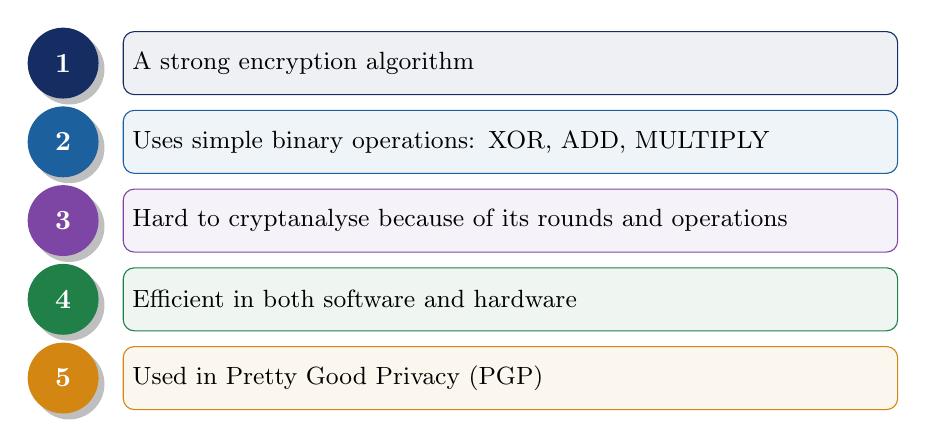
\begin{tikzpicture}
    \foreach \t/\c [count=\i from 0] in {A strong encryption algorithm/navy,Uses simple binary operations: XOR\comma{} ADD\comma{} MULTIPLY/ocean,Hard to cryptanalyse because of its rounds and operations/grape,Efficient in both software and hardware/leaf!80!black,Used in Pretty Good Privacy (PGP)/amber!90!black}{
      \node[circle,fill=\c,text=white,font=\bfseries,minimum size=9mm,drop shadow] (c\i) at (0,-\i*1.0) {\the\numexpr\i+1\relax};
      \node[draw=\c,fill=\c!7,rounded corners=4pt,anchor=west,text width=96mm,minimum height=8mm,font=\small] at ([xshift=3mm]c\i.east) {\t};
    }
  \end{tikzpicture}
\end{frame}

% ============================================================
\setcounter{section}{13}
\section{Advanced Encryption Standard}
% ============================================================

\begin{frame}{Why a New Standard?}
  \begin{columns}[c]
    \begin{column}{0.48\textwidth}
      \centering
      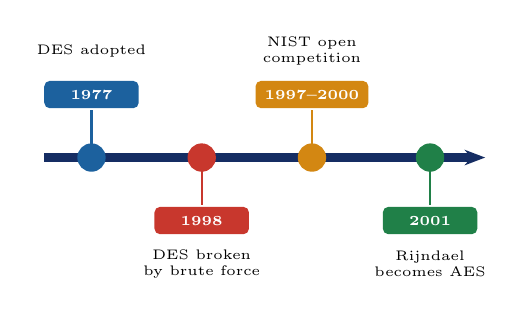
\begin{tikzpicture}
        \draw[navy,line width=3pt,->] (0,0) -- (5.6,0);
        \foreach \x/\c/\y/\t/\d in {0.6/ocean/1/1977/DES adopted,2.0/brick/-1/1998/DES broken\\by brute force,3.4/amber!90!black/1/1997--2000/NIST open\\competition,4.9/leaf!80!black/-1/2001/Rijndael\\becomes AES}{
          \fill[\c] (\x,0) circle (1.8mm); \draw[\c,thick] (\x,0) -- (\x,\y*0.6);
          \node[fill=\c,text=white,rounded corners=2pt,font=\tiny\bfseries,minimum width=12mm] at (\x,\y*0.8) {\t};
          \node[font=\tiny,align=center] at (\x,\y*1.35) {\d};
        }
      \end{tikzpicture}
    \end{column}
    \begin{column}{0.5\textwidth}
      \begin{itemize}\small\setlength{\itemsep}{3pt}
        \item DES's \textbf{56-bit key} became too short; triple DES was secure but \textbf{slow}
        \item NIST ran an open competition for a replacement
        \item The winner, \textbf{Rijndael} (Daemen and Rijmen), became the \textbf{Advanced Encryption Standard (AES)}
        \item Being \textbf{royalty-free} was a key selection criterion (recall Module 5)
      \end{itemize}
    \end{column}
  \end{columns}
\end{frame}

% ------------------------------------------------------------
\begin{frame}{AES Parameters}
  \centering
  \renewcommand{\arraystretch}{1.45}
  \begin{tabular}{>{\bfseries}l >{\columncolor{ocean!8}}c >{\columncolor{grape!8}}c >{\columncolor{brick!8}}c}
    \toprule
    \rowcolor{navy}\textcolor{white}{Key size} & \textcolor{white}{\textbf{128 bits}} & \textcolor{white}{\textbf{192 bits}} & \textcolor{white}{\textbf{256 bits}}\\
    \midrule
    Block size & 128 bits & 128 bits & 128 bits\\
    Number of rounds & \textbf{10} & \textbf{12} & \textbf{14}\\
    Round key size & 128 bits & 128 bits & 128 bits\\
    Expanded key & 44 words & 52 words & 60 words\\
    \bottomrule
  \end{tabular}
  \vspace{4mm}
  \begin{block}{Compare with DES}
    \small Twice the block size, and at least $2^{72}$ times more keys. AES is \textbf{not a Feistel cipher}: every round transforms the \textbf{whole block}, not just half.
  \end{block}
\end{frame}

% ------------------------------------------------------------
\begin{frame}{The State: AES Thinks in a 4 $\times$ 4 Grid}
  \begin{columns}[c]
    \begin{column}{0.5\textwidth}
      \centering
      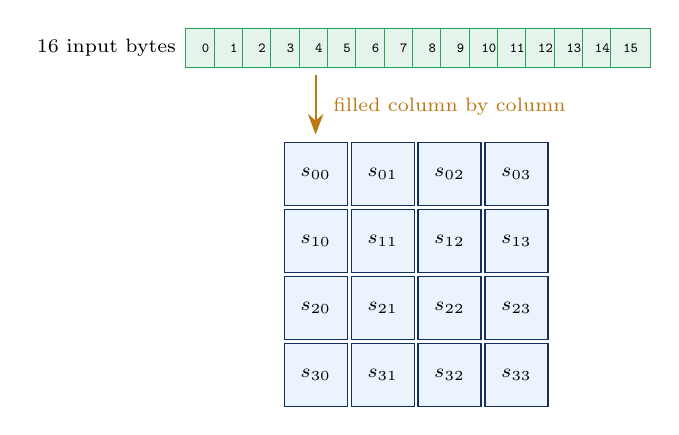
\begin{tikzpicture}
        \foreach \i in {0,...,15} \node[draw=leaf,fill=leaf!12,minimum size=5mm,font=\tiny\ttfamily] at (\i*0.36-2.7,1.6) {\i};
        \node[font=\scriptsize,anchor=east] at (-2.95,1.6) {16 input bytes};
        \foreach \r in {0,...,3} \foreach \c in {0,...,3}{
          \pgfmathtruncatemacro{\v}{\c*4+\r}
          \node[draw=navy,fill=sky,minimum size=8mm,font=\scriptsize\ttfamily] at (\c*0.85-1.3,-\r*0.85) {$s_{\r\c}$};
        }
        \draw[->,thick,amber!80!black] (-1.3,1.25) -- (-1.3,0.5);
        \node[font=\scriptsize,text=amber!80!black] at (0.4,0.85) {filled column by column};
      \end{tikzpicture}
    \end{column}
    \begin{column}{0.48\textwidth}
      \begin{itemize}\small\setlength{\itemsep}{4pt}
        \item The 128-bit block (16 bytes) is copied into a $4 \times 4$ array of bytes called the \textbf{State}
        \item Bytes fill the State \textbf{column by column}
        \item Every transformation changes the State; at the end it is copied out as the ciphertext
        \item The key is also arranged as a matrix of bytes and expanded into \textbf{words} (4 bytes each)
      \end{itemize}
    \end{column}
  \end{columns}
\end{frame}

% ------------------------------------------------------------
\begin{frame}{AES Cipher: Overall Structure}
  \begin{columns}[c]
    \begin{column}{0.52\textwidth}
      \centering
      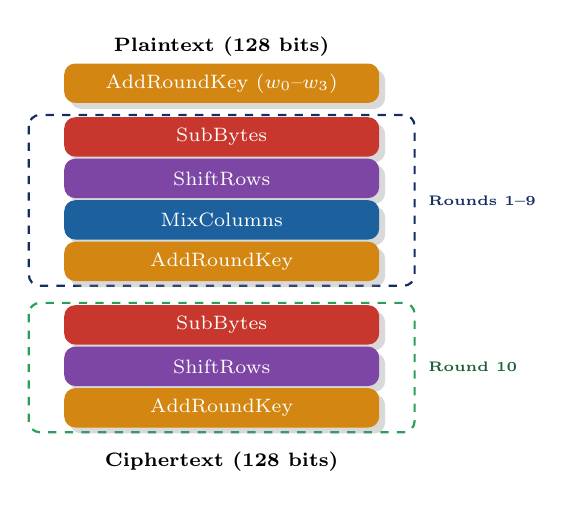
\begin{tikzpicture}[y=0.62cm]
        \node[font=\scriptsize\bfseries] at (0,0.75) {Plaintext (128 bits)};
        \node[solid box=amber!90!black,minimum width=40mm,minimum height=5mm,font=\scriptsize] at (0,0) {AddRoundKey ($w_0$--$w_3$)};
        \draw[navy,dashed,thick,rounded corners] (-2.45,-0.65) rectangle (2.45,-4.15);
        \node[font=\tiny\bfseries,text=navy,anchor=west] at (2.5,-2.4) {Rounds 1--9};
        \foreach \t/\c/\y in {SubBytes/brick/-1.1,ShiftRows/grape/-1.95,MixColumns/ocean/-2.8,AddRoundKey/amber!90!black/-3.65}
          \node[solid box=\c,minimum width=40mm,minimum height=5mm,font=\scriptsize] at (0,\y) {\t};
        \draw[leaf,dashed,thick,rounded corners] (-2.45,-4.5) rectangle (2.45,-7.15);
        \node[font=\tiny\bfseries,text=leaf!60!black,anchor=west] at (2.5,-5.8) {Round 10};
        \foreach \t/\c/\y in {SubBytes/brick/-4.95,ShiftRows/grape/-5.8,AddRoundKey/amber!90!black/-6.65}
          \node[solid box=\c,minimum width=40mm,minimum height=5mm,font=\scriptsize] at (0,\y) {\t};
        \node[font=\scriptsize\bfseries] at (0,-7.75) {Ciphertext (128 bits)};
\end{tikzpicture}
    \end{column}
    \begin{column}{0.46\textwidth}
      \begin{itemize}\small\setlength{\itemsep}{3pt}
        \item Begins with an \textbf{AddRoundKey} stage
        \item Then $N$ rounds; for a 128-bit key, $N = 10$
        \item Each full round has \textbf{four stages}
        \item The \textbf{last round omits MixColumns}
      \end{itemize}
      \begin{block}{One permutation, three substitutions}
        \small ShiftRows is a permutation; SubBytes, MixColumns and AddRoundKey are substitutions. Only \textbf{AddRoundKey} uses the key.
      \end{block}
    \end{column}
  \end{columns}
\end{frame}

% ------------------------------------------------------------
\begin{frame}{The Four Transformations at a Glance}
  \centering
  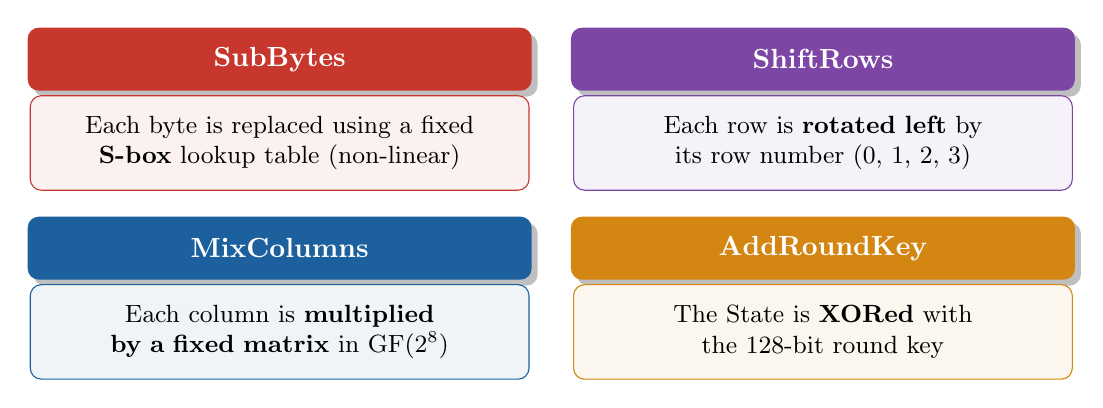
\begin{tikzpicture}
    \foreach \x/\y/\c/\t/\d in {
      0/0/brick/SubBytes/Each byte is replaced using a fixed \textbf{S-box} lookup table (non-linear),
      6.9/0/grape/ShiftRows/Each row is \textbf{rotated left} by its row number (0\comma{} 1\comma{} 2\comma{} 3),
      0/-2.4/ocean/MixColumns/Each column is \textbf{multiplied by a fixed matrix} in GF($2^8$),
      6.9/-2.4/amber!90!black/AddRoundKey/The State is \textbf{XORed} with the 128-bit round key}
    {
      \node[fill=\c,text=white,rounded corners=4pt,font=\bfseries,minimum width=64mm,minimum height=8mm,drop shadow] (h) at (\x,\y) {\t};
      \node[draw=\c,fill=\c!7,rounded corners=4pt,text width=61mm,minimum height=12mm,font=\small,anchor=north,align=center] at ([yshift=-0.5mm]h.south) {\d};
    }
  \end{tikzpicture}
  \vspace{2mm}

  {\small Each has a \textbf{forward} form (for encryption) and an \textbf{inverse} form (for decryption).}
\end{frame}

% ------------------------------------------------------------
\begin{frame}{Substitute Bytes Transformation}
  \begin{columns}[c]
    \begin{column}{0.52\textwidth}
      \centering
      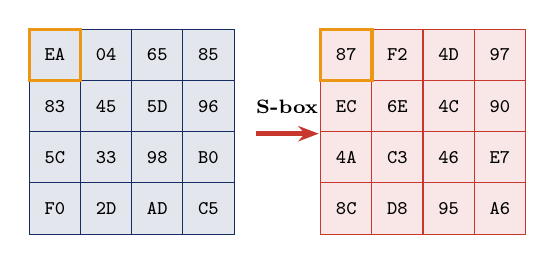
\begin{tikzpicture}
        \stategrid{0}{0}{navy}{EA,04,65,85,83,45,5D,96,5C,33,98,B0,F0,2D,AD,C5}
        \draw[flow=brick,line width=2pt] (2.55,-1.0) -- node[above=1mm,font=\scriptsize\bfseries]{S-box} (3.35,-1.0);
        \stategrid{3.7}{0}{brick}{87,F2,4D,97,EC,6E,4C,90,4A,C3,46,E7,8C,D8,95,A6}
        \node[draw=amber,very thick,minimum size=6.5mm] at (0,0) {};
        \node[draw=amber,very thick,minimum size=6.5mm] at (3.7,0) {};
      \end{tikzpicture}\\[3mm]
      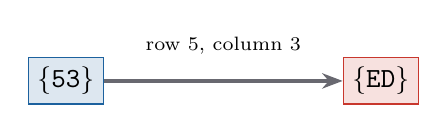
\begin{tikzpicture}
        \node[fill=ocean!15,draw=ocean,font=\ttfamily\bfseries] (in) at (0,0) {\{53\}};
        \node[font=\scriptsize,align=center] at (2.0,0.45) {row 5, column 3};
        \node[fill=brick!15,draw=brick,font=\ttfamily\bfseries] (out) at (4,0) {\{ED\}};
        \draw[flow] (in) -- (out);
      \end{tikzpicture}
    \end{column}
    \begin{column}{0.46\textwidth}
      \begin{block}{Forward transformation}
        \small A simple \textbf{table lookup}. AES defines a $16 \times 16$ S-box of byte values. For each State byte, the \textbf{left 4 bits} pick the row and the \textbf{right 4 bits} pick the column.
      \end{block}
      \begin{block}{Inverse transformation}
        \small Uses the \textbf{inverse S-box}: InvSubBytes maps \{ED\} back to \{53\}.
      \end{block}
    \end{column}
  \end{columns}
\end{frame}

% ------------------------------------------------------------
\begin{frame}{SubBytes: Rationale}
  \centering
  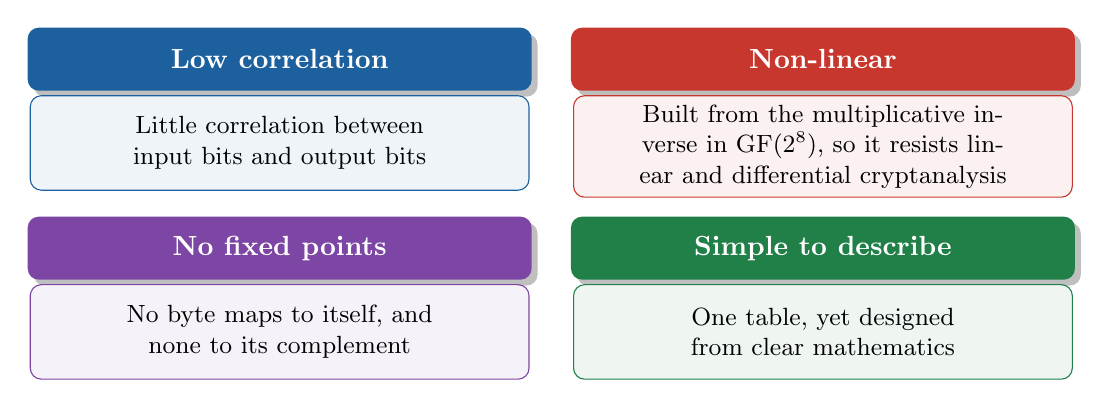
\begin{tikzpicture}
    \foreach \t/\d/\c [count=\i from 0] in {
      Low correlation/Little correlation between input bits and output bits/ocean,
      Non-linear/Built from the multiplicative inverse in GF($2^8$)\comma{} so it resists linear and differential cryptanalysis/brick,
      No fixed points/No byte maps to itself\comma{} and none to its complement/grape,
      Simple to describe/One table\comma{} yet designed from clear mathematics/leaf!80!black}
    {
      \pgfmathsetmacro{\x}{mod(\i,2)*6.9}
      \pgfmathsetmacro{\y}{-floor(\i/2)*2.4}
      \node[fill=\c,text=white,rounded corners=4pt,font=\bfseries,minimum width=64mm,minimum height=8mm,drop shadow] (h) at (\x,\y) {\t};
      \node[draw=\c,fill=\c!7,rounded corners=4pt,text width=61mm,minimum height=12mm,font=\small,anchor=north,align=center] at ([yshift=-0.5mm]h.south) {\d};
    }
  \end{tikzpicture}
  \vspace{2mm}

  {\small The S-box is the \textbf{only non-linear} step in AES, just as the S-boxes were in DES.}
\end{frame}

% ------------------------------------------------------------
\begin{frame}{ShiftRows Transformation}
  \begin{columns}[c]
    \begin{column}{0.54\textwidth}
      \centering
      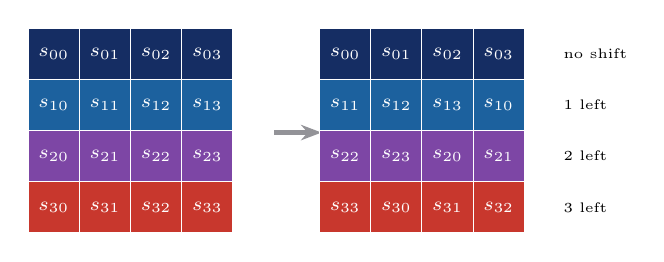
\begin{tikzpicture}
        \foreach \r/\c in {0/navy,1/ocean,2/grape,3/brick}
          \foreach \k in {0,...,3} \node[draw=white,fill=\c,text=white,minimum size=6.5mm,font=\scriptsize\ttfamily] at (\k*0.65,-\r*0.65) {$s_{\r\k}$};
        \draw[flow=ink!50,line width=2pt] (2.8,-1.0) -- (3.4,-1.0);
        \foreach \r/\c in {0/navy,1/ocean,2/grape,3/brick}
          \foreach \k in {0,...,3}{
            \pgfmathtruncatemacro{\src}{mod(\k+\r,4)}
            \node[draw=white,fill=\c,text=white,minimum size=6.5mm,font=\scriptsize\ttfamily] at (3.7+\k*0.65,-\r*0.65) {$s_{\r\src}$};
          }
        \foreach \r/\t in {0/no shift,1/1 left,2/2 left,3/3 left} \node[font=\tiny,anchor=west] at (6.35,-\r*0.65) {\t};
      \end{tikzpicture}
    \end{column}
    \begin{column}{0.44\textwidth}
      \begin{block}{Forward ShiftRows}
        \small Row 0 is not changed. Row 1 is rotated \textbf{1 byte left}, row 2 \textbf{2 bytes}, row 3 \textbf{3 bytes}.
      \end{block}
      \begin{block}{Inverse ShiftRows}
        \small The same shifts, but to the \textbf{right}.
      \end{block}
      \begin{exampleblock}{Rationale}
        \small The 4 bytes of one column are \textbf{spread to four different columns}. Without this, AES would be four independent ciphers.
      \end{exampleblock}
    \end{column}
  \end{columns}
\end{frame}

% ------------------------------------------------------------
\begin{frame}{MixColumns Transformation}
  \begin{columns}[c]
    \begin{column}{0.56\textwidth}
      \centering
      $\begin{bmatrix} 02 & 03 & 01 & 01\\ 01 & 02 & 03 & 01\\ 01 & 01 & 02 & 03\\ 03 & 01 & 01 & 02 \end{bmatrix}
      \begin{bmatrix} s_{0j}\\ s_{1j}\\ s_{2j}\\ s_{3j} \end{bmatrix} =
      \begin{bmatrix} s'_{0j}\\ s'_{1j}\\ s'_{2j}\\ s'_{3j} \end{bmatrix}$\\[4mm]
      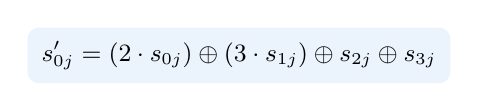
\begin{tikzpicture}
        \node[fill=sky,rounded corners,font=\small,align=left,inner sep=5pt] {$s'_{0j} = (2 \cdot s_{0j}) \oplus (3 \cdot s_{1j}) \oplus s_{2j} \oplus s_{3j}$};
      \end{tikzpicture}
    \end{column}
    \begin{column}{0.42\textwidth}
      \begin{block}{Forward MixColumns}
        \small Works on each \textbf{column} separately. Each byte is replaced by a function of \textbf{all four bytes} in its column: a matrix multiplication in GF($2^8$), where ``+'' is XOR.
      \end{block}
      \begin{block}{Inverse MixColumns}
        \small Multiply by the inverse matrix, with entries \{0E\}, \{0B\}, \{0D\}, \{09\}.
      \end{block}
    \end{column}
  \end{columns}
\end{frame}

% ------------------------------------------------------------
\begin{frame}{MixColumns: Rationale}
  \begin{columns}[c]
    \begin{column}{0.46\textwidth}
      \centering
      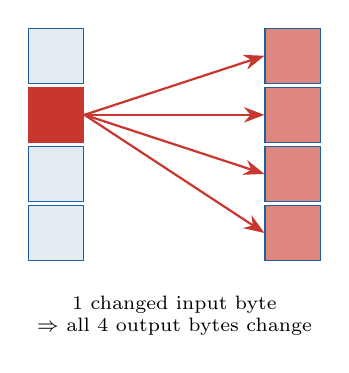
\begin{tikzpicture}
        \foreach \r in {0,...,3} \node[draw=ocean,fill=ocean!12,minimum size=7mm] (a\r) at (0,-\r*0.75) {};
        \fill[brick] (a1.south west) rectangle (a1.north east);
        \foreach \r in {0,...,3} {\node[draw=ocean,fill=brick!60,minimum size=7mm] (b\r) at (3,-\r*0.75) {}; \draw[->,brick,thick] (a1.east) -- (b\r.west);}
        \node[font=\scriptsize,align=center] at (1.5,-3.3) {1 changed input byte\\$\Rightarrow$ all 4 output bytes change};
      \end{tikzpicture}
    \end{column}
    \begin{column}{0.52\textwidth}
      \begin{itemize}\small\setlength{\itemsep}{4pt}
        \item Gives good \textbf{mixing among the bytes} of each column
        \item Combined with ShiftRows, after a few rounds \textbf{every output bit depends on every input bit}
        \item Coefficients \{01\}, \{02\}, \{03\} make it fast: multiplying by 2 is a shift and a conditional XOR
      \end{itemize}
      \begin{alertblock}{Why skip it in the last round?}
        \small It makes the cipher and its inverse look alike, and adds no security at the very end.
      \end{alertblock}
    \end{column}
  \end{columns}
\end{frame}

% ------------------------------------------------------------
\begin{frame}{AddRoundKey Transformation}
  \centering
  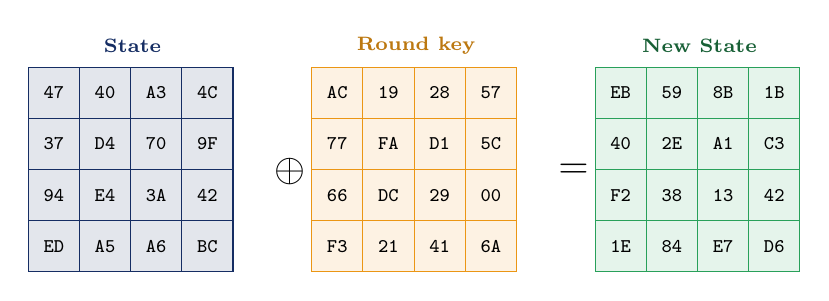
\begin{tikzpicture}
    \stategrid{0}{0}{navy}{47,40,A3,4C,37,D4,70,9F,94,E4,3A,42,ED,A5,A6,BC}
    \node[font=\Large\bfseries] at (3.0,-1.0) {$\oplus$};
    \stategrid{3.6}{0}{amber}{AC,19,28,57,77,FA,D1,5C,66,DC,29,00,F3,21,41,6A}
    \node[font=\Large\bfseries] at (6.6,-1.0) {$=$};
    \stategrid{7.2}{0}{leaf}{EB,59,8B,1B,40,2E,A1,C3,F2,38,13,42,1E,84,E7,D6}
    \node[font=\scriptsize\bfseries,text=navy] at (1.0,0.6) {State};
    \node[font=\scriptsize\bfseries,text=amber!80!black] at (4.6,0.6) {Round key};
    \node[font=\scriptsize\bfseries,text=leaf!60!black] at (8.2,0.6) {New State};
  \end{tikzpicture}
  \vspace{3mm}
  \begin{columns}[T]
    \begin{column}{0.48\textwidth}
      \begin{block}{Forward and inverse}
        \small The 128 bits of the State are \textbf{XORed} with the 128 bits of the round key. XOR is its own inverse, so the inverse is the \textbf{same operation}.
      \end{block}
    \end{column}
    \begin{column}{0.48\textwidth}
      \begin{exampleblock}{Rationale}
        \small As simple as possible, yet it affects \textbf{every bit}. The key expansion's complexity plus the other stages give the security.
      \end{exampleblock}
    \end{column}
  \end{columns}
\end{frame}

% ------------------------------------------------------------
\begin{frame}{AES Key Expansion}
  \begin{columns}[c]
    \begin{column}{0.54\textwidth}
      \centering
      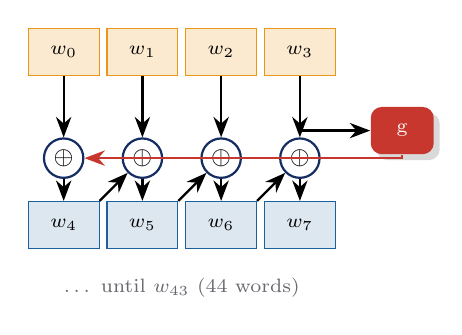
\begin{tikzpicture}
        \foreach \i in {0,...,3} \node[draw=amber,fill=amber!20,minimum width=9mm,minimum height=6mm,font=\scriptsize] (w\i) at (\i*1.0,0) {$w_\i$};
        \foreach \i in {4,...,7} \node[draw=ocean,fill=ocean!15,minimum width=9mm,minimum height=6mm,font=\scriptsize] (w\i) at (\i*1.0-4,-2.2) {$w_\i$};
        \node[solid box=brick,minimum width=8mm,minimum height=6mm,font=\scriptsize] (g) at (4.3,-1.0) {g};
        \draw[->,thick] (w3.south) |- (g.west);
        \foreach \i/\p in {4/0,5/1,6/2,7/3}{
          \node[xorn] (x\i) at (\i-4,-1.35) {$\oplus$};
          \draw[->,thick] (w\p) -- (x\i); \draw[->,thick] (x\i) -- (w\i);
        }
        \draw[->,thick,brick] (g.south) |- (x4.east);
        \foreach \i/\j in {4/5,5/6,6/7} \draw[->,thick] (w\i.north east) -- (x\j.south west);
        \node[font=\scriptsize,text=ink!70] at (1.5,-3.0) {\dots\ until $w_{43}$ (44 words)};
      \end{tikzpicture}
    \end{column}
    \begin{column}{0.44\textwidth}
      \begin{itemize}\small\setlength{\itemsep}{3pt}
        \item The 16-byte key fills the first 4 words $w_0$--$w_3$
        \item Each new word: $w_i = w_{i-1} \oplus w_{i-4}$
        \item For every \textbf{4th} word, $w_{i-1}$ first goes through \textbf{g}
      \end{itemize}
      \begin{block}{The function g}
        \small 1.~\textbf{RotWord}: rotate the 4 bytes left by one\\
        2.~\textbf{SubWord}: S-box on each byte\\
        3.~XOR with a round constant \textbf{Rcon}: 01, 02, 04, 08, 10, 20, 40, 80, 1B, 36
      \end{block}
    \end{column}
  \end{columns}
\end{frame}

% ------------------------------------------------------------
\begin{frame}{Key Expansion: Rationale}
  \centering
  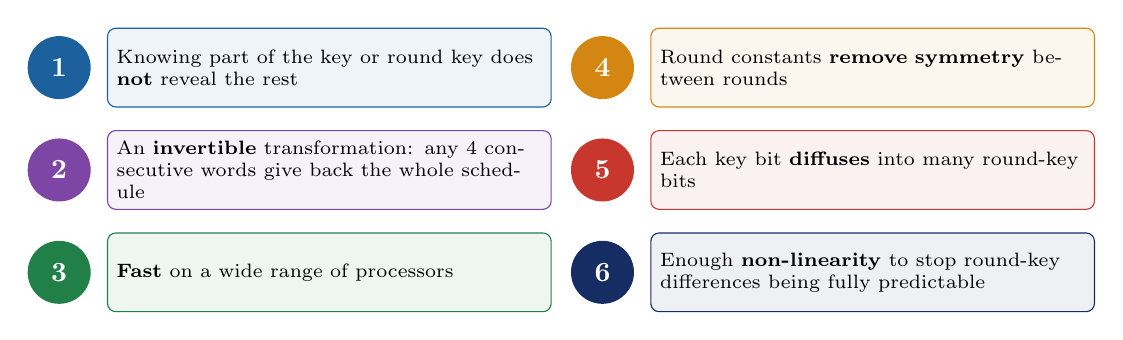
\begin{tikzpicture}
    \foreach \t/\c [count=\i] in {
      Knowing part of the key or round key does \textbf{not} reveal the rest/ocean,
      An \textbf{invertible} transformation: any 4 consecutive words give back the whole schedule/grape,
      \textbf{Fast} on a wide range of processors/leaf!80!black,
      Round constants \textbf{remove symmetry} between rounds/amber!90!black,
      Each key bit \textbf{diffuses} into many round-key bits/brick,
      Enough \textbf{non-linearity} to stop round-key differences being fully predictable/navy}
    {
      \pgfmathsetmacro{\x}{ifthenelse(\i<4,0,6.9)}
      \pgfmathsetmacro{\y}{-mod(\i-1,3)*1.3}
      \node[circle,fill=\c,text=white,font=\bfseries,minimum size=8mm] (c\i) at (\x,\y) {\i};
      \node[draw=\c,fill=\c!7,rounded corners=3pt,anchor=west,text width=54mm,minimum height=10mm,font=\scriptsize] at ([xshift=2mm]c\i.east) {\t};
    }
  \end{tikzpicture}
  \vspace{3mm}
  \begin{block}{Design goal}
    \small Resist known attacks, especially attacks where the attacker knows or can control \textbf{part of the key}.
  \end{block}
\end{frame}

% ------------------------------------------------------------
\begin{frame}{Equivalent Inverse Cipher}
  \begin{columns}[c]
    \begin{column}{0.54\textwidth}
      \centering
      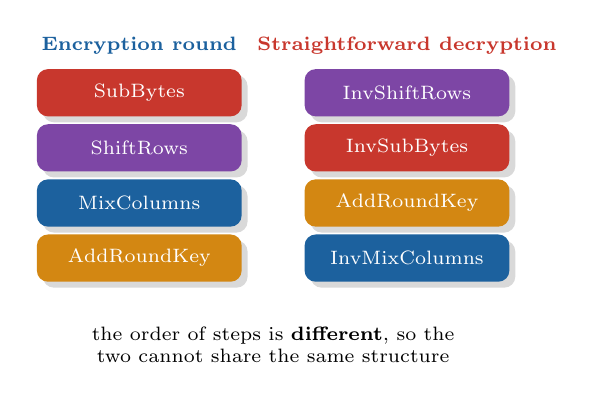
\begin{tikzpicture}
        \node[font=\scriptsize\bfseries,text=ocean] at (0,2.4) {Encryption round};
        \node[font=\scriptsize\bfseries,text=brick] at (3.4,2.4) {Straightforward decryption};
        \foreach \t/\c [count=\i from 0] in {SubBytes/brick,ShiftRows/grape,MixColumns/ocean,AddRoundKey/amber!90!black}
          \node[solid box=\c,minimum width=26mm,minimum height=6mm,font=\scriptsize] at (0,1.8-\i*0.7) {\t};
        \foreach \t/\c [count=\i from 0] in {InvShiftRows/grape,InvSubBytes/brick,AddRoundKey/amber!90!black,InvMixColumns/ocean}
          \node[solid box=\c,minimum width=26mm,minimum height=6mm,font=\scriptsize] at (3.4,1.8-\i*0.7) {\t};
        \node[font=\scriptsize,text width=60mm,align=center] at (1.7,-1.4) {the order of steps is \textbf{different}, so the two cannot share the same structure};
      \end{tikzpicture}
    \end{column}
    \begin{column}{0.44\textwidth}
      \begin{itemize}\small\setlength{\itemsep}{4pt}
        \item The straightforward decryption cipher uses the inverse steps in a \textbf{different order}
        \item For efficiency, we want decryption to have the \textbf{same structure} as encryption
        \item Two swaps make this possible, giving the \textbf{equivalent inverse cipher}
      \end{itemize}
      \begin{block}{Benefit}
        \small The same hardware or code layout can be used for both directions.
      \end{block}
    \end{column}
  \end{columns}
\end{frame}

% ------------------------------------------------------------
\begin{frame}{The Two Interchanges}
  \begin{columns}[T]
    \begin{column}{0.49\textwidth}
      \centering\textbf{\textcolor{grape}{InvShiftRows $\leftrightarrow$ InvSubBytes}}\\[2mm]
      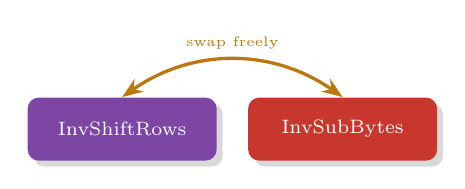
\begin{tikzpicture}
        \node[solid box=grape,minimum width=24mm,font=\scriptsize] (a) at (0,0) {InvShiftRows};
        \node[solid box=brick,minimum width=24mm,font=\scriptsize] (b) at (2.8,0) {InvSubBytes};
        \draw[<->,very thick,amber!80!black] (a.north) to[bend left=35] node[above,font=\tiny]{swap freely} (b.north);
      \end{tikzpicture}\\[2mm]
      {\small InvShiftRows moves bytes \textbf{without changing} them; InvSubBytes changes bytes \textbf{without moving} them. So their order does not matter.}
    \end{column}
    \begin{column}{0.49\textwidth}
      \centering\textbf{\textcolor{ocean}{AddRoundKey $\leftrightarrow$ InvMixColumns}}\\[2mm]
      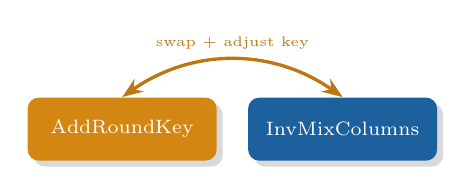
\begin{tikzpicture}
        \node[solid box=amber!90!black,minimum width=24mm,font=\scriptsize] (a) at (0,0) {AddRoundKey};
        \node[solid box=ocean,minimum width=24mm,font=\scriptsize] (b) at (2.8,0) {InvMixColumns};
        \draw[<->,very thick,amber!80!black] (a.north) to[bend left=35] node[above,font=\tiny]{swap + adjust key} (b.north);
      \end{tikzpicture}\\[2mm]
      {\small InvMixColumns is \textbf{linear}: $\mathrm{InvMix}(S \oplus K) = \mathrm{InvMix}(S) \oplus \mathrm{InvMix}(K)$. So swap them and apply InvMixColumns to the \textbf{round key} as well.}
    \end{column}
  \end{columns}
  \vspace{4mm}
  \begin{block}{Result}
    \small Decryption becomes: InvSubBytes, InvShiftRows, InvMixColumns, AddRoundKey with modified keys: the \textbf{same layout} as encryption.
  \end{block}
\end{frame}

% ------------------------------------------------------------
\begin{frame}{DES vs.\ IDEA vs.\ AES}
  \centering
  \renewcommand{\arraystretch}{1.45}
  \small
  \begin{tabular}{>{\bfseries}l >{\columncolor{ocean!8}}c >{\columncolor{grape!8}}c >{\columncolor{brick!8}}c}
    \toprule
    \rowcolor{navy}\textcolor{white}{Feature} & \textcolor{white}{\textbf{DES}} & \textcolor{white}{\textbf{IDEA}} & \textcolor{white}{\textbf{AES}}\\
    \midrule
    Block size & 64 bits & 64 bits & 128 bits\\
    Key size & 56 bits & 128 bits & 128 / 192 / 256 bits\\
    Rounds & 16 & 8 + output transf. & 10 / 12 / 14\\
    Structure & Feistel & Mixed algebraic groups & Substitution--permutation\\
    Non-linearity from & 8 S-boxes & Multiply* mod $2^{16}{+}1$ & One byte S-box\\
    Status & Broken by brute force & Used in PGP & Current standard\\
    \bottomrule
  \end{tabular}
\end{frame}

% ============================================================
\setcounter{section}{14}
\section{Modes of Operation}
% ============================================================

\begin{frame}{Why Do We Need Modes of Operation?}
  \begin{columns}[c]
    \begin{column}{0.5\textwidth}
      \centering
      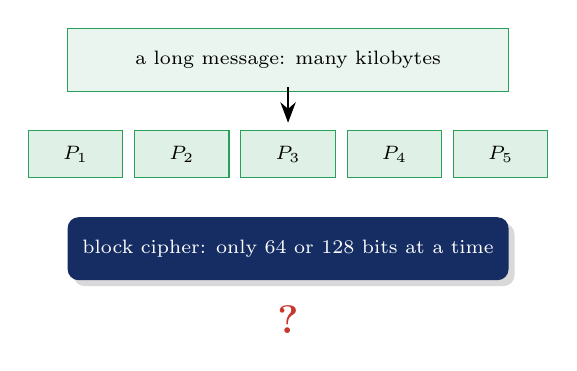
\begin{tikzpicture}
        \node[draw=leaf,fill=leaf!10,minimum width=56mm,minimum height=8mm,font=\scriptsize] at (0,1.2) {a long message: many kilobytes};
        \foreach \i in {0,...,4} \node[blk] (b\i) at (\i*1.35-2.7,0) {$P_{\the\numexpr\i+1\relax}$};
        \draw[->,thick] (0,0.85) -- (0,0.4);
        \node[solid box=navy,minimum width=56mm,minimum height=8mm,font=\scriptsize] at (0,-1.2) {block cipher: only 64 or 128 bits at a time};
        \node[font=\Large\bfseries,text=brick] at (0,-2.1) {?};
      \end{tikzpicture}
    \end{column}
    \begin{column}{0.48\textwidth}
      \begin{itemize}\small\setlength{\itemsep}{4pt}
        \item A block cipher encrypts \textbf{one fixed-size block}
        \item Real messages are much \textbf{longer}
        \item A \textbf{mode of operation} says how to apply the cipher to a sequence of blocks
        \item The last block may need \textbf{padding} to fill it
      \end{itemize}
      \begin{block}{Four block cipher modes}
        \small \textbf{ECB}, \textbf{CBC}, \textbf{CFB}, \textbf{OFB}
      \end{block}
    \end{column}
  \end{columns}
\end{frame}

% ------------------------------------------------------------
\begin{frame}{Electronic Code Book (ECB) Mode}
  \centering
  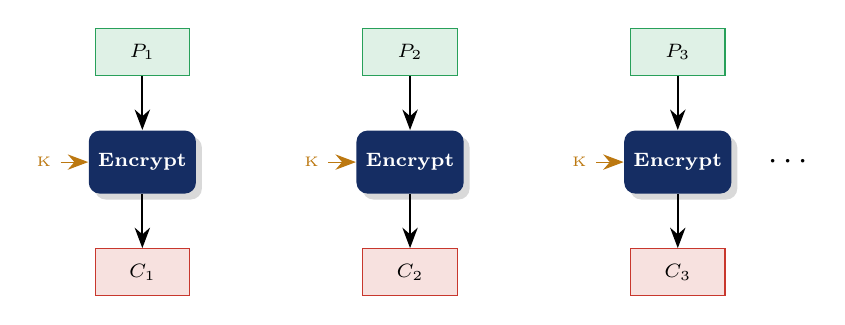
\begin{tikzpicture}
    \foreach \i in {1,2,3} {
      \node[blk] (p\i) at (\i*3.4,1.4) {$P_\i$};
      \node[ek] (e\i) at (\i*3.4,0) {Encrypt};
      \node[blk=brick] (c\i) at (\i*3.4,-1.4) {$C_\i$};
      \draw[->,thick] (p\i) -- (e\i); \draw[->,thick] (e\i) -- (c\i);
      \node[font=\tiny,text=amber!80!black] (k\i) at (\i*3.4-1.25,0) {K};
      \draw[->,amber!80!black] (k\i) -- (e\i);
    }
    \node[font=\large] at (11.6,0) {$\cdots$};
  \end{tikzpicture}
  \vspace{3mm}
  \begin{columns}[T]
    \begin{column}{0.48\textwidth}
      \begin{block}{How it works}
        \small Each block is encrypted \textbf{independently} with the same key: $C_i = E_K(P_i)$. Like a code book: every plaintext block has its own ciphertext entry.
      \end{block}
    \end{column}
    \begin{column}{0.48\textwidth}
      \begin{alertblock}{Weakness}
        \small \textbf{Identical plaintext blocks give identical ciphertext blocks}, so patterns show through. Good only for short data, such as a single key.
      \end{alertblock}
    \end{column}
  \end{columns}
\end{frame}


% ------------------------------------------------------------
\begin{frame}{ECB Leaks Patterns}
  \centering
  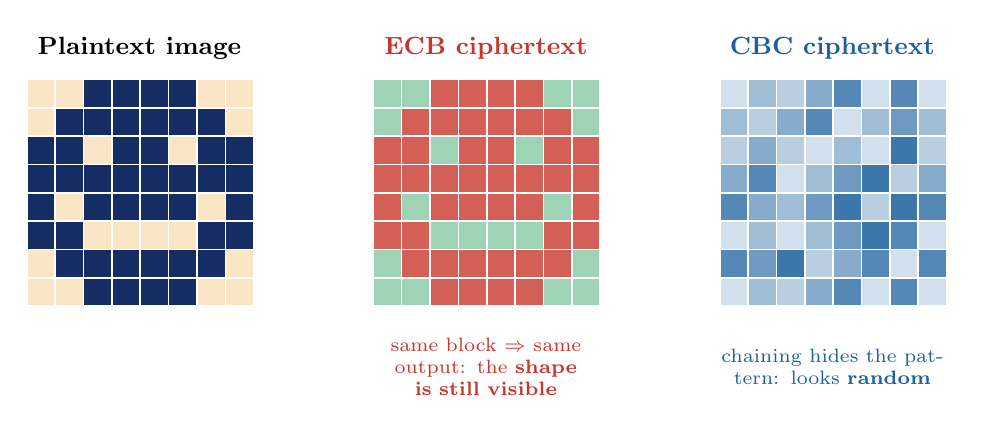
\begin{tikzpicture}
    \def\pat{{0,0,1,1,1,1,0,0, 0,1,1,1,1,1,1,0, 1,1,0,1,1,0,1,1, 1,1,1,1,1,1,1,1, 1,0,1,1,1,1,0,1, 1,1,0,0,0,0,1,1, 0,1,1,1,1,1,1,0, 0,0,1,1,1,1,0,0}}
    \foreach \k in {0,...,63}{
      \pgfmathtruncatemacro{\r}{\k/8}\pgfmathtruncatemacro{\c}{mod(\k,8)}\pgfmathtruncatemacro{\v}{\pat[\k]}
      \ifnum\v=1 \fill[navy] (\c*0.36,-\r*0.36) rectangle ++(0.34,0.34); \else \fill[amber!25] (\c*0.36,-\r*0.36) rectangle ++(0.34,0.34); \fi
      \ifnum\v=1 \fill[brick!80] (4.4+\c*0.36,-\r*0.36) rectangle ++(0.34,0.34); \else \fill[leaf!45] (4.4+\c*0.36,-\r*0.36) rectangle ++(0.34,0.34); \fi
      \pgfmathtruncatemacro{\h}{mod(\k*37+\v*11,7)}
      \fill[ocean!\the\numexpr 20+\h*11\relax] (8.8+\c*0.36,-\r*0.36) rectangle ++(0.34,0.34);
    }
    \node[font=\small\bfseries] at (1.42,0.75) {Plaintext image};
    \node[font=\small\bfseries,text=brick] at (5.82,0.75) {ECB ciphertext};
    \node[font=\small\bfseries,text=ocean] at (10.22,0.75) {CBC ciphertext};
    \node[font=\scriptsize,text=brick,text width=34mm,align=center] at (5.82,-3.3) {same block $\Rightarrow$ same output: the \textbf{shape is still visible}};
    \node[font=\scriptsize,text=ocean,text width=34mm,align=center] at (10.22,-3.3) {chaining hides the pattern: looks \textbf{random}};
  \end{tikzpicture}
  \vspace{2mm}

  {\small Each small square stands for one block. ECB turns each distinct block into its own distinct colour, so the picture survives encryption.}
\end{frame}

% ------------------------------------------------------------
\begin{frame}{Cipher Block Chaining (CBC) Mode}
  \centering
  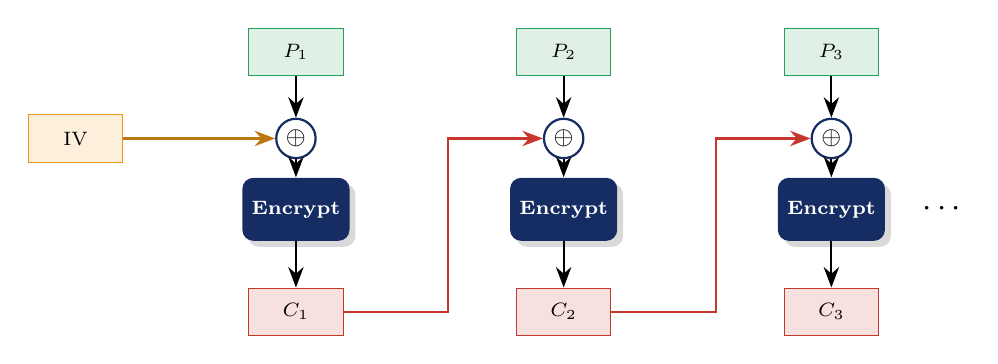
\begin{tikzpicture}
    \node[blk=amber] (iv) at (0.6,0.9) {IV};
    \foreach \i in {1,2,3} {
      \node[blk] (p\i) at (\i*3.4,2.0) {$P_\i$};
      \node[xorn] (x\i) at (\i*3.4,0.9) {$\oplus$};
      \node[ek] (e\i) at (\i*3.4,0) {Encrypt};
      \node[blk=brick] (c\i) at (\i*3.4,-1.3) {$C_\i$};
      \draw[->,thick] (p\i) -- (x\i); \draw[->,thick] (x\i) -- (e\i); \draw[->,thick] (e\i) -- (c\i);
    }
    \draw[->,thick,amber!80!black] (iv) -- (x1);
    \draw[->,thick,brick] (c1.east) -| ([xshift=-12mm]x2.west) -- (x2.west);
    \draw[->,thick,brick] (c2.east) -| ([xshift=-12mm]x3.west) -- (x3.west);
    \node[font=\large] at (11.6,0) {$\cdots$};
  \end{tikzpicture}
  \vspace{3mm}
  \begin{columns}[T]
    \begin{column}{0.48\textwidth}
      \begin{block}{How it works}
        \small Each plaintext block is \textbf{XORed with the previous ciphertext block} before encryption: $C_i = E_K(P_i \oplus C_{i-1})$, with $C_0 = $ an \textbf{Initialization Vector (IV)}.
      \end{block}
    \end{column}
    \begin{column}{0.48\textwidth}
      \begin{exampleblock}{Benefit}
        \small Identical plaintext blocks now give \textbf{different} ciphertext. Decryption: $P_i = D_K(C_i) \oplus C_{i-1}$. Widely used for bulk data and authentication.
      \end{exampleblock}
    \end{column}
  \end{columns}
\end{frame}


% ------------------------------------------------------------
\begin{frame}{CBC Decryption}
  \centering
  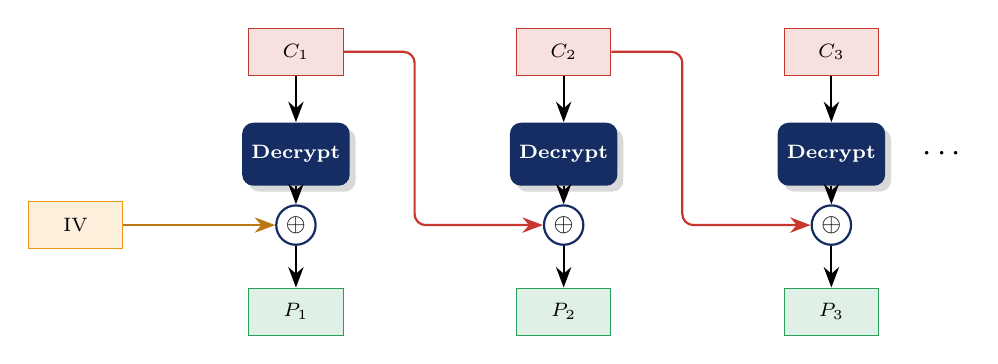
\begin{tikzpicture}
    \node[blk=amber] (iv) at (0.6,-0.9) {IV};
    \foreach \i in {1,2,3} {
      \node[blk=brick] (c\i) at (\i*3.4,1.3) {$C_\i$};
      \node[ek] (d\i) at (\i*3.4,0) {Decrypt};
      \node[xorn] (x\i) at (\i*3.4,-0.9) {$\oplus$};
      \node[blk] (p\i) at (\i*3.4,-2.0) {$P_\i$};
      \draw[->,thick] (c\i) -- (d\i); \draw[->,thick] (d\i) -- (x\i); \draw[->,thick] (x\i) -- (p\i);
    }
    \draw[->,thick,amber!80!black] (iv) -- (x1);
    \draw[->,thick,brick,rounded corners] (c1.east) -- ++(0.9,0) |- (x2.west);
    \draw[->,thick,brick,rounded corners] (c2.east) -- ++(0.9,0) |- (x3.west);
    \node[font=\large] at (11.6,0) {$\cdots$};
  \end{tikzpicture}
  \vspace{3mm}
  \begin{columns}[T]
    \begin{column}{0.48\textwidth}
      \begin{block}{Formula}
        \small $P_i = D_K(C_i) \oplus C_{i-1}$, with $C_0 = $ IV. Each block is decrypted, then XORed with the \textbf{previous ciphertext} block.
      \end{block}
    \end{column}
    \begin{column}{0.48\textwidth}
      \begin{alertblock}{Error propagation}
        \small A bit error in $C_i$ garbles all of $P_i$ and flips \textbf{one bit} of $P_{i+1}$. After that, decryption recovers.
      \end{alertblock}
    \end{column}
  \end{columns}
\end{frame}

% ------------------------------------------------------------
\begin{frame}{The Initialization Vector (IV)}
  \begin{columns}[c]
    \begin{column}{0.46\textwidth}
      \centering
      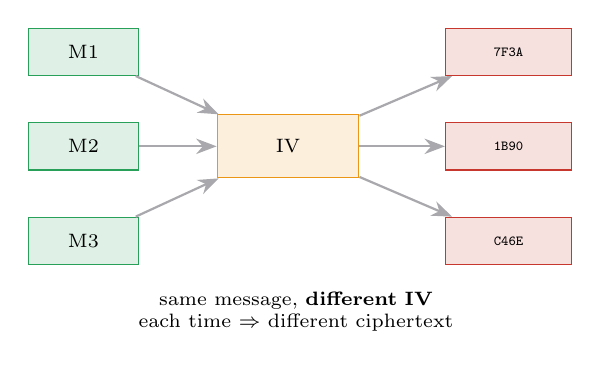
\begin{tikzpicture}
        \node[blk=amber,minimum width=18mm,minimum height=8mm] (iv) at (0,0) {IV};
        \foreach \m/\y in {M1/1.2,M2/0,M3/-1.2} {\node[blk,minimum width=14mm] (m) at (-2.6,\y) {\m}; \draw[->,thick,ink!40] (m) -- (iv);}
        \foreach \c/\y/\v in {C1/1.2/7F3A,C2/0/1B90,C3/-1.2/C46E} {\node[blk=brick,minimum width=16mm,font=\tiny\ttfamily] (c) at (2.8,\y) {\v}; \draw[->,thick,ink!40] (iv) -- (c);}
        \node[font=\scriptsize,text width=50mm,align=center] at (0.1,-2.1) {same message, \textbf{different IV} each time $\Rightarrow$ different ciphertext};
      \end{tikzpicture}
    \end{column}
    \begin{column}{0.52\textwidth}
      \begin{itemize}\small\setlength{\itemsep}{4pt}
        \item CBC, CFB and OFB need a starting value, the \textbf{IV}, to begin the chain
        \item The IV must be known to \textbf{both sender and receiver}
        \item It does not need to be secret, but it must be \textbf{protected from change} and should be \textbf{unpredictable}
        \item Using a fresh IV means encrypting the same message twice gives \textbf{different ciphertexts}
      \end{itemize}
      \begin{alertblock}{OFB warning}
        \small Never reuse the same key and IV in OFB: it would repeat the key stream.
      \end{alertblock}
    \end{column}
  \end{columns}
\end{frame}

% ------------------------------------------------------------
\begin{frame}{Cipher Feedback (CFB) Mode}
  \centering
  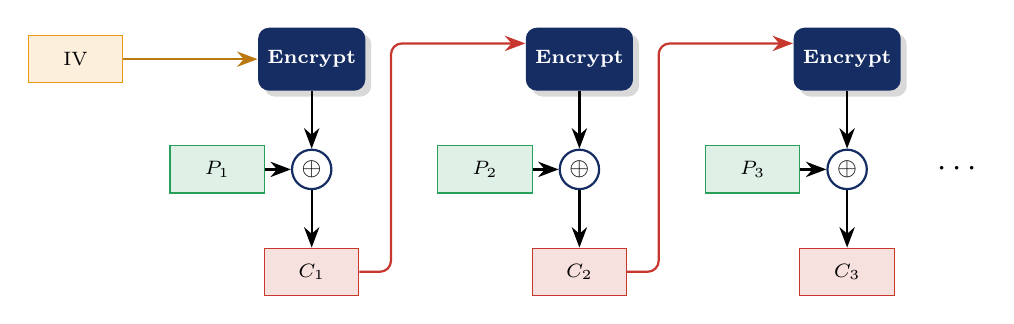
\begin{tikzpicture}
    \node[blk=amber] (iv) at (0.4,1.4) {IV};
    \foreach \i in {1,2,3} {
      \node[ek] (e\i) at (\i*3.4,1.4) {Encrypt};
      \node[blk] (p\i) at (\i*3.4-1.2,0) {$P_\i$};
      \node[xorn] (x\i) at (\i*3.4,0) {$\oplus$};
      \node[blk=brick] (c\i) at (\i*3.4,-1.3) {$C_\i$};
      \draw[->,thick] (e\i) -- (x\i); \draw[->,thick] (p\i) -- (x\i); \draw[->,thick] (x\i) -- (c\i);
    }
    \draw[->,thick,amber!80!black] (iv) -- (e1);
    \draw[->,thick,brick,rounded corners] (c1.east) -- ++(0.4,0) |- ([yshift=2mm]e2.west);
    \draw[->,thick,brick,rounded corners] (c2.east) -- ++(0.4,0) |- ([yshift=2mm]e3.west);
    \node[font=\large] at (11.6,0) {$\cdots$};
  \end{tikzpicture}
  \vspace{3mm}
  \begin{columns}[T]
    \begin{column}{0.48\textwidth}
      \begin{block}{How it works}
        \small The \textbf{previous ciphertext} is encrypted, and the result is XORed with the plaintext: $C_i = P_i \oplus E_K(C_{i-1})$. Can work on small units (e.g.\ 8 bits) at a time.
      \end{block}
    \end{column}
    \begin{column}{0.48\textwidth}
      \begin{exampleblock}{Key property}
        \small Turns a block cipher into a \textbf{self-synchronizing stream cipher}. Decryption uses the \textbf{encrypt} function too. Good for character-by-character data.
      \end{exampleblock}
    \end{column}
  \end{columns}
\end{frame}

% ------------------------------------------------------------
\begin{frame}{Output Feedback (OFB) Mode}
  \centering
  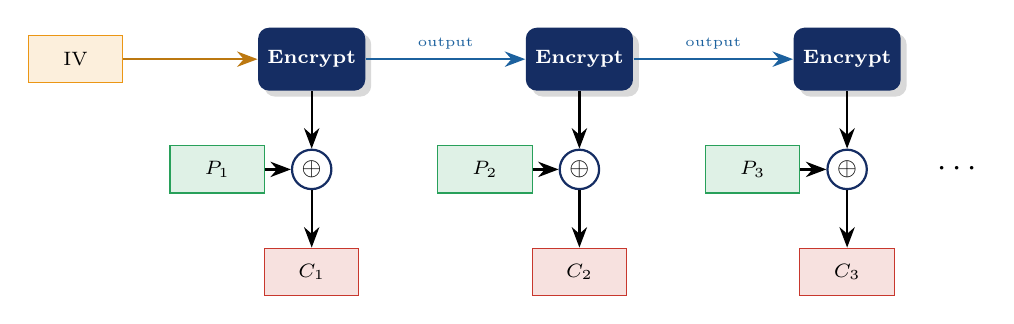
\begin{tikzpicture}
    \node[blk=amber] (iv) at (0.4,1.4) {IV};
    \foreach \i in {1,2,3} {
      \node[ek] (e\i) at (\i*3.4,1.4) {Encrypt};
      \node[blk] (p\i) at (\i*3.4-1.2,0) {$P_\i$};
      \node[xorn] (x\i) at (\i*3.4,0) {$\oplus$};
      \node[blk=brick] (c\i) at (\i*3.4,-1.3) {$C_\i$};
      \draw[->,thick] (e\i) -- (x\i); \draw[->,thick] (p\i) -- (x\i); \draw[->,thick] (x\i) -- (c\i);
    }
    \draw[->,thick,amber!80!black] (iv) -- (e1);
    \draw[->,thick,ocean] (e1) -- node[above,font=\tiny]{output} (e2);
    \draw[->,thick,ocean] (e2) -- node[above,font=\tiny]{output} (e3);
    \node[font=\large] at (11.6,0) {$\cdots$};
  \end{tikzpicture}
  \vspace{3mm}
  \begin{columns}[T]
    \begin{column}{0.48\textwidth}
      \begin{block}{How it works}
        \small Like CFB, but the \textbf{output of the encryption function} (not the ciphertext) is fed back. The key stream does not depend on the message.
      \end{block}
    \end{column}
    \begin{column}{0.48\textwidth}
      \begin{exampleblock}{Key property}
        \small A \textbf{bit error} in one ciphertext block affects \textbf{only that bit} of plaintext; errors do not spread. Good for noisy channels such as satellite links.
      \end{exampleblock}
    \end{column}
  \end{columns}
\end{frame}

% ------------------------------------------------------------
\begin{frame}{CFB vs.\ OFB: What Is Fed Back?}
  \begin{columns}[T]
    \begin{column}{0.49\textwidth}
      \centering\textbf{\textcolor{brick}{CFB: ciphertext is fed back}}\\[2mm]
      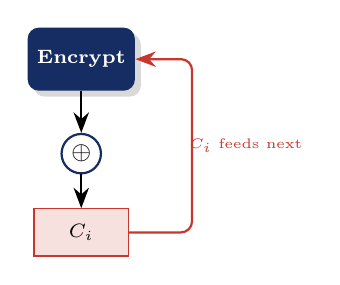
\begin{tikzpicture}
        \node[ek] (e) at (0,0) {Encrypt};
        \node[xorn] (x) at (0,-1.2) {$\oplus$};
        \node[blk=brick] (c) at (0,-2.2) {$C_i$};
        \draw[->,thick] (e) -- (x); \draw[->,thick] (x) -- (c);
        \draw[->,thick,brick,rounded corners] (c.east) -- ++(0.8,0) |- (e.east);
        \node[font=\tiny,text=brick,anchor=west] at (1.25,-1.1) {$C_i$ feeds next};
      \end{tikzpicture}\\[2mm]
      {\small An error in $C_i$ also garbles the \textbf{next} block(s).}
    \end{column}
    \begin{column}{0.49\textwidth}
      \centering\textbf{\textcolor{ocean}{OFB: cipher output is fed back}}\\[2mm]
      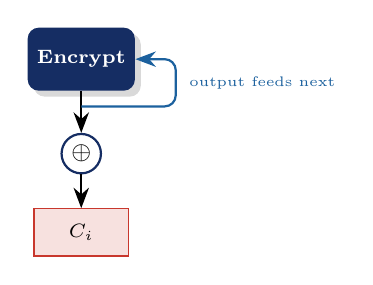
\begin{tikzpicture}
        \node[ek] (e) at (0,0) {Encrypt};
        \node[xorn] (x) at (0,-1.2) {$\oplus$};
        \node[blk=brick] (c) at (0,-2.2) {$C_i$};
        \draw[->,thick] (e) -- (x); \draw[->,thick] (x) -- (c);
        \draw[->,thick,ocean,rounded corners] (0,-0.6) -- ++(1.2,0) |- (e.east);
        \node[font=\tiny,text=ocean,anchor=west] at (1.25,-0.3) {output feeds next};
      \end{tikzpicture}\\[2mm]
      {\small An error in $C_i$ affects \textbf{only} that block. But OFB is more open to message-stream \textbf{modification}.}
    \end{column}
  \end{columns}
\end{frame}

% ------------------------------------------------------------
\begin{frame}{Comparing the Four Modes}
  \centering
  \renewcommand{\arraystretch}{1.45}
  \small
  \begin{tabular}{>{\bfseries}l >{\raggedright\arraybackslash}p{3.6cm} >{\raggedright\arraybackslash}p{3.0cm} >{\raggedright\arraybackslash}p{3.2cm}}
    \toprule
    \rowcolor{navy}\textcolor{white}{Mode} & \textcolor{white}{\textbf{Description}} & \textcolor{white}{\textbf{Same $P$ $\Rightarrow$ same $C$?}} & \textcolor{white}{\textbf{Typical use}}\\
    \midrule
    \textcolor{ocean}{ECB} & Each block encrypted independently & \bad{Yes} & Short data, e.g.\ a key\\
    \textcolor{grape}{CBC} & XOR with previous ciphertext, then encrypt & \good{No} & Bulk data, authentication\\
    \textcolor{brick}{CFB} & Encrypt previous ciphertext, XOR with plaintext & \good{No} & Stream data, characters\\
    \textcolor{leaf!70!black}{OFB} & Encrypt previous cipher output, XOR with plaintext & \good{No} & Noisy channels (satellite)\\
    \bottomrule
  \end{tabular}
\end{frame}

% ------------------------------------------------------------
\begin{frame}{Quick Check}
  \centering
  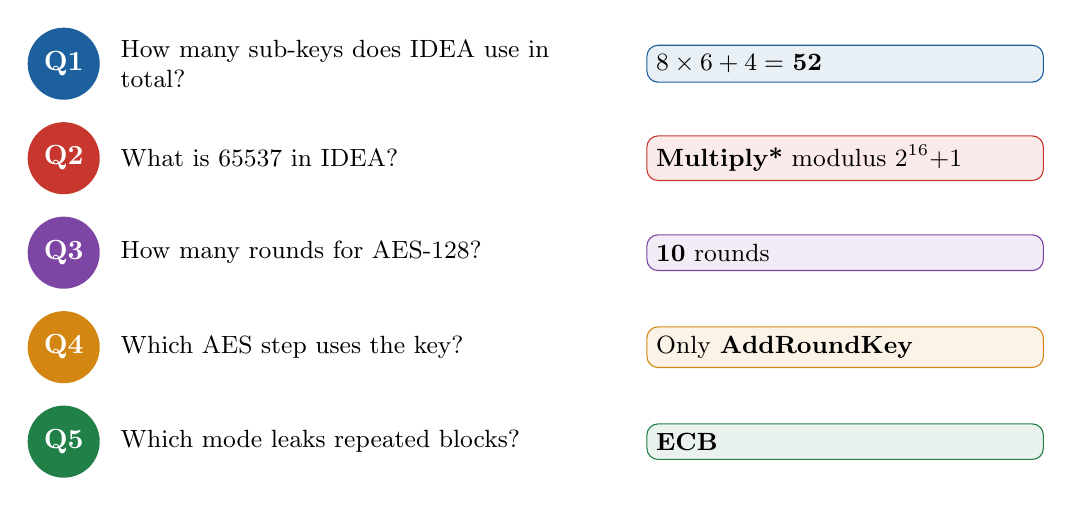
\begin{tikzpicture}
    \foreach \q/\a/\c [count=\i] in {
      How many sub-keys does IDEA use in total?/$8 \times 6 + 4 = $ \textbf{52}/ocean,
      What is $65537$ in IDEA?/\textbf{Multiply*} modulus $2^{16}{+}1$/brick,
      How many rounds for AES-128?/\textbf{10} rounds/grape,
      Which AES step uses the key?/Only \textbf{AddRoundKey}/amber!90!black,
      Which mode leaks repeated blocks?/\textbf{ECB}/leaf!80!black}
    {
      \node[circle,fill=\c,text=white,font=\bfseries,minimum size=8mm] (n\i) at (0,-\i*1.2) {Q\i};
      \node[anchor=west,font=\small,text width=60mm] at (0.6,-\i*1.2) {\q};
      \node[anchor=west,fill=\c!10,draw=\c,rounded corners,font=\small,text width=48mm] at (7.4,-\i*1.2) {\a};
    }
  \end{tikzpicture}
\end{frame}

% ------------------------------------------------------------
\begin{frame}{Module 7 Summary}
  \begin{columns}[T]
    \begin{column}{0.32\textwidth}
      \begin{block}{Lesson 13: IDEA}
        \scriptsize
        \begin{itemize}\setlength{\itemsep}{0pt}
          \item 64-bit block, 128-bit key
          \item XOR, Add*, Multiply*
          \item 8 rounds $\times$ 6 + 4 = 52 sub-keys
          \item 25-bit key shifting
          \item Output transformation
          \item Inverse sub-keys decrypt
        \end{itemize}
      \end{block}
    \end{column}
    \begin{column}{0.32\textwidth}
      \begin{alertblock}{Lesson 14: AES}
        \scriptsize
        \begin{itemize}\setlength{\itemsep}{0pt}
          \item 128-bit block; 10/12/14 rounds
          \item SubBytes, ShiftRows
          \item MixColumns, AddRoundKey
          \item Key expansion: RotWord, SubWord, Rcon
          \item Equivalent inverse cipher
        \end{itemize}
      \end{alertblock}
    \end{column}
    \begin{column}{0.32\textwidth}
      \begin{exampleblock}{Lesson 15: Modes}
        \scriptsize
        \begin{itemize}\setlength{\itemsep}{0pt}
          \item ECB: independent blocks
          \item CBC: chain with IV
          \item CFB: ciphertext feedback
          \item OFB: output feedback
        \end{itemize}
      \end{exampleblock}
    \end{column}
  \end{columns}
  \vspace{2mm}
  \begin{alertblock}{Review questions}
    \small
    1.~Give a brief account of IDEA. \quad 2.~Explain the structure of AES and its four transformations. \quad
    3.~Explain AES key expansion. \quad 4.~Explain the ECB, CBC, CFB and OFB modes with diagrams.
  \end{alertblock}
\end{frame}

% ------------------------------------------------------------
\begin{frame}{References}
  \begin{enumerate}\setlength{\itemsep}{8pt}
    \item William Stallings, \emph{Cryptography and Network Security}, PHI Publishers.
    \item Charlie Kaufman, Radia Perlman, \emph{Network Security}, Pearson Education.
    \item Bruce Schneier, \emph{Applied Cryptography}, John Wiley \& Sons.
    \item Roberta Bragg, \emph{Network Security: The Complete Reference}, TMH.
  \end{enumerate}
  \vspace{6mm}
  \centering
  
\begin{tikzpicture}
    \node[fill=navy,text=white,rounded corners=8pt,inner sep=10pt,font=\Large\bfseries,drop shadow] {Thank You! \; Questions?};
  \end{tikzpicture}
\end{frame}

\end{document}
